% !TeX program = xelatex
% !TeX encoding = UTF-8
\documentclass[12pt,a4paper]{article}
\usepackage[margin=2.5cm]{geometry}
\usepackage{amsmath,amssymb,amsthm,xeCJK,graphicx}
\usepackage[hidelinks]{hyperref}
\usepackage{fancyhdr,enumitem,needspace,longtable}
\setCJKmainfont{Microsoft JhengHei}
\setCJKmonofont{Microsoft JhengHei}
\makeatletter
\newcommand{\totalpages}{\@abspage@last}
\makeatother
\pagestyle{fancy}
\fancyhf{}
\renewcommand{\headrulewidth}{0pt}
\fancyfoot[C]{\thepage/\totalpages}
\fancypagestyle{plain}{\fancyhf{}\renewcommand{\headrulewidth}{0pt}\fancyfoot[C]{\thepage/\totalpages}}
\setlength{\parindent}{0pt}
\setlength{\parskip}{4pt}
\setlist{nosep,topsep=5pt}
\newcommand{\editorial}[1]{\par\smallskip{\small\textbf{編輯註：}#1}\par}

\newsavebox{\questionbox}
\newlength{\questionroom}
\newenvironment{questionprompt}{%
  \begin{lrbox}{\questionbox}\begin{minipage}{\linewidth}%
}{%
  \end{minipage}\end{lrbox}%
  \setlength{\questionroom}{\dimexpr\ht\questionbox+\dp\questionbox+5.2cm\relax}%
  \ifdim\questionroom>\textheight\setlength{\questionroom}{\textheight}\fi
  \Needspace{\questionroom}%
  \noindent\usebox{\questionbox}\par
}

\title{Linear System --- Textbook Practice for Midterm}
\author{葉彥辰\\P46154345}
\date{}
\begin{document}
\maketitle
本練習集依教材 \texttt{linearsys\_note.pdf} 的 Exercise 整理。
教師未公告明確範圍，以下依 HW1--HW5 的實際主題推估：第 2--7 章為主，
另含第 9 章脈衝響應 Exercise 108；第 8 章 Exercise 107 為選做延伸。
不納入第 10 章以後的穩定性、Lyapunov、可觀測性與控制器設計。

前 30 題是第一輪題型巡迴：每種主要題型先練一題，依估計手算量與整合程度由淺入深排列，
不按教材章節順序。第 31--109 題為第二輪，將剩餘題目隨機打散，包含較長與綜合題。
計算量是相對估計；證明題所需時間也會因熟悉程度而異。
每題下方保留原題號與教材印刷頁碼。
教材 PDF 的實體頁碼為印刷頁碼加 8。
原書重複題仍保留，Exercise 11/12 因原書編號混排而合併。
原 Exercise 61 為純 MATLAB 數值實驗，略去；Exercise 109 涉及 Lyapunov 方程，略去。

所有題目只需手算。模擬、程式與畫圖要求已刪除或改為求解析響應。
部分題目調整為較容易計算的數值，均註明「數值調整版」；
一般符號題與原本適合手算的數字保留。
原書缺符號、編號混排或未明訂條件之處，均採明確標註的練習版本；不需等待原書勘誤。

每題的 Solution 僅留空白；可在原始碼中直接輸入答案並自行增減留白。
\bigskip
\textbf{題目總數：109 題組（含 1 題選做）。}
\clearpage


\section*{第一輪：題型巡迴路線}
先完成第 1--30 題，讓主要單元各練習一輪，再進入第二輪隨機練習。
\begin{longtable}{r p{11cm}}
\textbf{題號}&\textbf{練習重點}\\\hline
1 & 基底與維度\\
2 & 線性映射\\
3 & 行列式性質證明\\
4 & 行列式與反矩陣\\
5 & 子空間證明\\
6 & 由特徵值建立伴隨矩陣\\
7 & 特徵多項式\\
8 & Cayley--Hamilton 與矩陣冪\\
9 & 離散遞迴與狀態變數\\
10 & 含延遲的轉移函數\\
11 & 線性方程組\\
12 & 值域與零空間\\
13 & 複數特徵結構\\
14 & 相似關係證明\\
15 & 特徵值與週期解證明\\
16 & 高階微分方程的狀態空間\\
17 & 零平衡點線性化\\
18 & 平衡點與線性化\\
19 & 座標轉換\\
20 & SISO 實現與最小性\\
21 & MIMO 輸入輸出實現\\
22 & 對角化\\
23 & 矩陣指數\\
24 & 一般矩陣函數\\
25 & 機械系統建模\\
26 & 耦合非線性系統建模\\
27 & 矩陣多項式計算\\
28 & 連續時間模態響應\\
29 & 離散時間模態響應\\
30 & 脈衝響應與模態激發\\
\end{longtable}\clearpage

\section*{第一輪：各題型由淺入深}

\begin{questionprompt}
\section*{Exercise 1}
\phantomsection\label{practice:1}
{\small Source: Exercise 55; textbook pp.~105.}\par
Give an example of a basis for $\mathbb R^3$ and for $\mathbb R^{2\times3}$. What are the dimensions of these spaces?
\end{questionprompt}
\subsection*{Solution}
% 在這裡撰寫解答。


I had finished.


\vspace{3.5cm}



\begin{questionprompt}
\section*{Exercise 2}
\phantomsection\label{practice:2}
{\small Source: Exercise 20; textbook pp.~48.}\par
Suppose $A$ and $B$ are fixed real $n\times n$ matrices and consider the map $L$ from $\mathbb R^{n\times n}$ to $\mathbb R^{n\times n}$ given by
\[L(P)=PA+BP\]
for any $n\times n$ matrix $P$. Show that $L$ is a linear map.
\end{questionprompt}
\subsection*{Solution}
% 在這裡撰寫解答。

Just need to proof that

\[
L(aP + bQ) = aL(P) + bL(Q)
\]


\vspace{3.5cm}


\begin{questionprompt}
\section*{Exercise 3}
\phantomsection\label{practice:3}
{\small Source: Exercise 16; textbook pp.~45.}\par
Prove that if $A$ is invertible then
\[\det(A^{-1})=\frac{1}{\det A}.\]
\end{questionprompt}
\subsection*{Solution}
% 在這裡撰寫解答。

I had done.
\vspace{3.5cm}


\begin{questionprompt}
\section*{Exercise 4}
\phantomsection\label{practice:4}
{\small Source: Exercise 15; textbook pp.~45.}\par
Compute the determinant and inverse of the following matrix.
\[\begin{bmatrix}\cos\theta&\sin\theta\\-\sin\theta&\cos\theta\end{bmatrix}.\]
\end{questionprompt}
\subsection*{Solution}
% 在這裡撰寫解答。

Determinant is 
\[
\begin{vmatrix}
	\cos \theta & \sin\theta\\-\sin\theta & \cos\theta
\end{vmatrix} = 1
\]

and

\[
\begin{bmatrix}\cos\theta&\sin\theta\\-\sin\theta&\cos\theta\end{bmatrix}^{-1} =\begin{bmatrix}\cos\theta&-\sin\theta\\ \sin\theta&\cos\theta\end{bmatrix}
\]

\vspace{3.5cm}


\begin{questionprompt}
\section*{Exercise 5}
\phantomsection\label{practice:5}
{\small Source: Exercise 53; textbook pp.~99.}\par
Show that $\operatorname{span}X$ is a subspace, where $X$ is a collection of vectors in a vector space and $\operatorname{span}X$ denotes all finite linear combinations of vectors in $X$.
\end{questionprompt}
\subsection*{Solution}
% 在這裡撰寫解答。

Skipped, due to I just need to practice calculation first.

\vspace{3.5cm}


\begin{questionprompt}
\section*{Exercise 6}
\phantomsection\label{practice:6}
{\small Source: Exercise 67; textbook pp.~130.}\par
What is the real $2\times2$ companion matrix with eigenvalues $1+j,1-j$?
\end{questionprompt}
\subsection*{Solution}
% 在這裡撰寫解答。
(I have no idea first)

\[
p(s) = (s- (1 + j)) (s - (1 -j)) = s^2-2s + 2 = a_2s^2 + a_1s + a_0
\]
\[
\Rightarrow \text{companion matrix} = \begin{bmatrix}
	0 & 1 \\ -a_0 & -a_1 
\end{bmatrix} = \begin{bmatrix}
0 & 1 \\ -2 & 2
\end{bmatrix}
\]



\vspace{3.5cm}


\begin{questionprompt}
\section*{Exercise 7}
\phantomsection\label{practice:7}
{\small Source: Exercise 65; textbook pp.~130.}\par
Compute the characteristic polynomial of
\[\begin{bmatrix}0&1\\-a_0&-a_1\end{bmatrix}.\]
Hence, write down the characteristic polynomials for the $A$ matrices associated with the unattached mass and the damped linear oscillator.
\editorial{補列原先參照模型，未代入狀態空間解答：unattached mass 為 $m\ddot q=u$；damped linear oscillator 為 $m\ddot q+c\dot q+kq=u$。}
\end{questionprompt}
\subsection*{Solution}
% 在這裡撰寫解答。
\vspace{3.5cm}


\begin{questionprompt}
\section*{Exercise 8}
\phantomsection\label{practice:8}
{\small Source: Exercise 90; textbook pp.~175.}\par
Without doing any matrix multiplications, compute $A^4$ for
\[A=\begin{bmatrix}0&1&0&0\\0&0&1&0\\0&0&0&1\\2&1&0&0\end{bmatrix}.\]
Justify your answer.
\editorial{數值調整版：原矩陣最後一列 $(564,1,0,0)$ 改為 $(2,1,0,0)$；保留兩個非零伴隨係數，需保留原題的 Cayley--Hamilton 判讀。}
\end{questionprompt}
\subsection*{Solution}
% 在這裡撰寫解答。

\begin{align*}
	\det (sI - A) &= \det\begin{bmatrix}
		s & -1 & 0 & 0 \\
		0 & s & -1 & 0 \\
		0 & 0 & s & -1 \\
		-2 & -1 & 0 & s
	\end{bmatrix} \\
	&= s \begin{vmatrix}
		s & -1 & 0 \\ 0 & s & -1 \\ -1 & 0 & s
	\end{vmatrix} +  2\begin{vmatrix}
	-1 & 0 & 0 \\ s & -1 & 0 \\ 0 & s & -1
	\end{vmatrix} \\
	&= s [ s (s^2) -1 ] -2 \\
	&= s^4 - s  - 2 = 0 \triangleq p(s) = 0
\end{align*}

Therefore
\[
p(A) = A^4 - A -2 = O \Rightarrow A^4 = A + 2I = \begin{bmatrix}2&1&0&0\\0&2&1&0\\0&0&2&1\\2&1&0&2\end{bmatrix}
\]

\vspace{3.5cm}


\begin{questionprompt}
\section*{Exercise 9}
\phantomsection\label{practice:9}
{\small Source: Exercise 7; textbook pp.~26.}\par
Consider the second order difference equation
\[q(k+2)=q(k+1)+q(k).\]
Obtain the solution corresponding to $q(0)=1$, $q(1)=1$ and $k=0,1,\ldots,10$. Obtain a state space description of this system.
\end{questionprompt}
\subsection*{Solution}
% 在這裡撰寫解答。

\[
x(k) = \begin{bmatrix}
	x_1(k) \\ x_2(k)
\end{bmatrix} = \begin{bmatrix}
	q(k) \\ q(k + 1)
\end{bmatrix}, x(k + 1) = \begin{bmatrix}
q(k + 1) \\ q(k + 2) 
\end{bmatrix} = \begin{bmatrix}
x_2(k) \\ x_1(k) + x_2(k)
\end{bmatrix} = \begin{bmatrix}
0 & 1 \\ 1 & 1
\end{bmatrix} x(k)
\]

\vspace{3.5cm}


\begin{questionprompt}
\section*{Exercise 10}
\phantomsection\label{practice:10}
{\small Source: Exercise 30; textbook pp.~71.}\par
What is the transfer function of the following system?
\[\dot x_1(t)=x_2(t),\qquad\dot x_2(t)=u(t-2),\qquad y(t)=x_1(t).\]
\end{questionprompt}
\subsection*{Solution}
% 在這裡撰寫解答。

From the condition that question gives

\[
s\hat x_1(s) = \hat x_2(s), \quad s\hat x_2(s) = e^{-2s}\hat u(s), \quad \hat y(s) =\hat x_1(s)
\]
Therefore 
\begin{align*}
	\hat y(s) &= \hat x_1(s) = {1\over s} \hat x_2(s)  \\
	&= {e^{-2s} \over s^2} \hat u(s)
\end{align*}

Finally the transfer function is

\[
\hat G(s) = {e^{-2s}\over s^2}
\]

\vspace{3.5cm}


\begin{questionprompt}
\section*{Exercise 11}
\phantomsection\label{practice:11}
{\small Source: Exercise 51; textbook pp.~97.}\par
Determine whether or not the following system of linear equations has a solution. If a solution exists, determine whether or not it is unique; if not unique, obtain an expression for all solutions and give two solutions.
\begin{align*}y-2z&=4\\x-y&=1\\3x-3y+4z&=-9\\-2y+10z&=-26\end{align*}
\end{questionprompt}
\subsection*{Solution}
% 在這裡撰寫解答。

\[
\begin{bmatrix}
	0 & 1 & -2 \\
	1 & -1 & 0 \\
	3 & -3 & 4 \\
	0 & -2 & 10
\end{bmatrix}\begin{bmatrix}
x \\ y \\ z
\end{bmatrix} = \begin{bmatrix}
4 \\ 1 \\ -9 \\ 26
\end{bmatrix} \overset{\text{Argu}}{\Rightarrow} \begin{bmatrix}
	0 & 1 & -2 & 4\\
1 & -1 & 0 & 1\\
3 & -3 & 4 & -9\\
0 & -2 & 10 & 26
\end{bmatrix}
\]

\begin{align*}
	&\begin{bmatrix}
		0 & 1 & -2 & 4\\
		1 & -1 & 0 & 1\\
		3 & -3 & 4 & -9\\
		0 & -2 & 10 & -26
	\end{bmatrix} \\
	\Rightarrow &\begin{bmatrix}
		1 & -1 & 0 & 1\\
		0 & 1 & -2 & 4\\
		3 & -3 & 4 & -9\\
		0 & -2 & 10 & -26
	\end{bmatrix} \\
	\Rightarrow &\begin{bmatrix}
		1 & -1 & 0 & 1\\
		0 & 1 & -2 & 4\\
		0 & 0 & 4 &  -12\\
		0 & -2 & 10 & -26
	\end{bmatrix} \\
		\Rightarrow &\begin{bmatrix}
		1 & -1 & 0 & 1\\
		0 & 1 & -2 & 4\\
		0 & 0 & 4 &  -12\\
		0 & 0 & 6 & 18
	\end{bmatrix} \\
	\Rightarrow &\begin{bmatrix}
		1 & -1 & 0 & 1\\
		0 & 1 & -2 & 4\\
		0 & 0 & 4 &  -12\\
		0 & 0 & 0 &  0
	\end{bmatrix} \Rightarrow \begin{bmatrix}
	1 & -1 & 0 & 1\\
	0 & 1 & -2 & 4\\
	0 & 0 & 1 &  -3\\
	0 & 0 & 0 & 0
	\end{bmatrix} \\
	\Rightarrow &\begin{bmatrix}
		1 & -1 & 0 & 1\\
		0 & 1 & 0 & -2\\
		0 & 0 & 1 &  -3\\
		0 & 0 & 0 & 0
	\end{bmatrix}\Rightarrow \begin{bmatrix}
	1 & 0 & 0 & -1\\
	0 & 1 &  0& -2\\
	0 & 0 & 1 &  -3\\
	0 & 0 & 0 & 0
	\end{bmatrix}  
\end{align*}

The only solution is $(x, y, z) = (-1, -2, -3)$


\vspace{3.5cm}


\begin{questionprompt}
\section*{Exercise 12}
\phantomsection\label{practice:12}
{\small Source: Exercise 56; textbook pp.~110.}\par
Find a basis for the range and the null space of each of the following matrices.
\[\begin{bmatrix}2&1\\2&1\end{bmatrix},\qquad\begin{bmatrix}1&-1\\1&-1\end{bmatrix}.\]
\editorial{原題為 ``Picturize the range and the null space''；改為求基底，不畫圖。}
\end{questionprompt}
\subsection*{Solution}
% 在這裡撰寫解答。

For $\begin{bmatrix}
	2 & 1 \\ 2 & 1
\end{bmatrix}$

Range is $\begin{bmatrix}
	1\\ 1
\end{bmatrix}$, and the null space is $\begin{bmatrix}
1 \\ -2
\end{bmatrix}$

For $\begin{bmatrix}
	1 & -1 \\ 1 & -1
\end{bmatrix}$

Range si $\begin{bmatrix}
	1 \\ 1
\end{bmatrix}$, and the null space is $\begin{bmatrix}
1 \\ 1
\end{bmatrix}$
\vspace{3.5cm}


\begin{questionprompt}
\section*{Exercise 13}
\phantomsection\label{practice:13}
{\small Source: Exercise 64; textbook pp.~127.}\par
Compute expressions for eigenvalues and linearly independent eigenvectors of
\[A=\begin{bmatrix}\alpha&\omega\\-\omega&\alpha\end{bmatrix},\qquad\alpha,\omega\ne0.\]
\end{questionprompt}
\subsection*{Solution}
% 在這裡撰寫解答。

\[
\det (sI - A) = \begin{vmatrix}
	s - \alpha & -\omega \\
	\omega & s - \alpha 
\end{vmatrix} = (s-\alpha)^2 + \omega^2 = 0 \Rightarrow s = \alpha \pm j\omega
\]

For $\lambda = \alpha + j\omega$

\[
(\lambda I - A)v = \begin{bmatrix}
	j\omega & -\omega \\ \omega & j\omega
\end{bmatrix}v = 0, \quad v = \begin{bmatrix}
1 \\ j
\end{bmatrix}
\]

For $\lambda = \alpha - j\omega$
\[
(\lambda I - A) v = \begin{bmatrix}
	-j\omega & -\omega \\ \omega & -j\omega  
\end{bmatrix}v = 0, \quad v = \begin{bmatrix}
1 \\ -j
\end{bmatrix}  
\]
\vspace{3.5cm}


\begin{questionprompt}
\section*{Exercise 14}
\phantomsection\label{practice:14}
{\small Source: Exercise 73; textbook pp.~149.}\par
Prove the following statements:
\begin{enumerate}[label=(\alph*)]
\item If $A$ is similar to $B$, then $B$ is similar to $A$.
\item If $A$ is similar to $B$ and $B$ is similar to $C$, then $A$ is similar to $C$.
\end{enumerate}
\end{questionprompt}
\subsection*{Solution}
% 在這裡撰寫解答。

If A is similar to B, so that $B = T^{-1}AT$, mutliply both side with $T$ and $T^{-1}$

\[
TBT^{-1} = A \overset{G = T^{-1}}{\Rightarrow} A = G^{-1} BG 
\]

Hence, B is similar to B also.

I am too lazy to write (b).

\vspace{3.5cm}


\begin{questionprompt}
\section*{Exercise 15}
\phantomsection\label{practice:15}
{\small Source: Exercise 96; textbook pp.~185.}\par
Consider $\dot x=Ax$, where $A$ is a square matrix. Show that if $A$ has $j2\pi$ as an eigenvalue, then there is a nonzero initial state $x_0$ such that the solution satisfies
\[x(1)=x(0)=x_0.\]
\end{questionprompt}
\subsection*{Solution}
% 在這裡撰寫解答。

\[
\dot x = Ax \Rightarrow x(t) = e^{At} x(0) = e^{At} x_0
\]
But if
\[
Av = \lambda v \Rightarrow x(t) = e^{\lambda t} v
\]


\vspace{3.5cm}


\begin{questionprompt}
\section*{Exercise 16}
\phantomsection\label{practice:16}
{\small Source: Exercise 1; textbook pp.~25.}\par
Consider a system described by a single $n$th-order linear differential equation
\[q^{(n)}+a_{n-1}q^{(n-1)}+\cdots+a_1\dot q+a_0q=0,\]
where $q(t)\in\mathbb R$ and $q^{(n)}:=d^nq/dt^n$. By appropriate definition of state variables, obtain a first order state space description of this system.
\end{questionprompt}
\subsection*{Solution}
% 在這裡撰寫解答。
\vspace{3.5cm}


\begin{questionprompt}
\section*{Exercise 17}
\phantomsection\label{practice:17}
{\small Source: Exercise 23; textbook pp.~59.}\par
Linearize each of the following systems about the zero equilibrium state.
\begin{enumerate}[label=(\roman*)]
\item $\dot x_1=(1+x_1^2)x_2,\quad\dot x_2=-x_1^3$.
\item $\dot x_1=\sin x_2,\quad\dot x_2=(\cos x_1)x_3,\quad\dot x_3=e^{x_1}x_2$.
\end{enumerate}
\end{questionprompt}
\subsection*{Solution}
% 在這裡撰寫解答。
(基本上OK 但是可能會有微小的計算錯誤
阿因為題目說 zero equilibrium state 所以 (ii) 的 $(\pi, 0, 0)$ 
暫時不列入考慮這樣
)
\subsubsection*{(i)}

\[
\begin{bmatrix}
	\dot x_1 \\ \dot x_2
\end{bmatrix} = \begin{bmatrix}
 	(1 + x_1^2) x_2 \\
 	-x_1^3
\end{bmatrix}
\]
At equilibrium state, $\dot x$ must be $0$. Therefore
\[
\begin{bmatrix}
	\dot x_1 \\ \dot x_2
\end{bmatrix} = \begin{bmatrix}
	(1 + x_1^2) x_2  \\
	-x_1^3
\end{bmatrix} = \begin{bmatrix}
0 \\ 0
\end{bmatrix} \quad \Rightarrow \begin{cases}
x^e_1 & = 0 \\
x^e_2 & = 0
\end{cases}
\]

Let 
\[
F(x) = \begin{bmatrix}
	F_1(x) \\ F_2(x) 
\end{bmatrix} = \begin{bmatrix}
(1 + x_1^2) x_2 \\ -x_1^3
\end{bmatrix}
\]

\begin{align*}
	A &= {\partial F \over \partial x} = \begin{bmatrix}
		{\partial F_1 \over \partial x_1} & {\partial F_1 \over \partial x_2} \\
		{\partial F_2 \over \partial x_2} & {\partial F_2 \over \partial x_2}
	\end{bmatrix} \\
	&= \begin{bmatrix}
		2x_1x_2 & 1 + x_1^2 \\
		0 & -3x_1^2
	\end{bmatrix}
\end{align*}

At equilibrium state
\[
A^e = A\bigg|_{x^e_1 = 0 , x_2^e = 0} = \begin{bmatrix}
	0 & 1 \\ 0 & 0
\end{bmatrix} \Rightarrow \delta \dot x = A^e \delta x
\]


\subsubsection*{(ii)}

\[
\begin{bmatrix}
	\dot x_1 \\ \dot x_2 \\ \dot x_3
\end{bmatrix} = \begin{bmatrix}
\sin x_2 \\ (\cos x_1) x_3 \\ e^{x_1} x_2
\end{bmatrix}
\]

At equilibrium state which means $\dot x = 0$

\[
\begin{bmatrix}
	\dot x_1 \\ \dot x_2 \\ \dot x_3
\end{bmatrix} = \begin{bmatrix}
	\sin x_2 \\ (\cos x_1) x_3 \\ e^{x_1} x_2
\end{bmatrix} = \begin{bmatrix}
0 \\ 0 \\ 0
\end{bmatrix} \Rightarrow \begin{cases}
x_1^e &= 0 \lor \pi \\
x_2^e &= 0 \\ 
x_3^e &= 0 
\end{cases}
\]

Let 
\[
F(x) = \begin{bmatrix}
	F_1 \\ F_2 \\ F_3
\end{bmatrix} = \begin{bmatrix}
\sin x_2 \\ (\cos x_1) x_3 \\ e^{x_1} x_2
\end{bmatrix}
\]
\begin{align*}
	A &= {\partial F \over \partial x} = \begin{bmatrix}
		{\partial F_1 \over \partial x_1} & {\partial F_1 \over \partial x_2} & {\partial F_1 \over \partial x_3} \\
		{\partial F_2 \over \partial x_1} & {\partial F_2 \over \partial x_2} & {\partial F_2 \over \partial x_3} \\
		{\partial F_3 \over \partial x_1} & {\partial F_3 \over \partial x_2} & {\partial F_3 \over \partial x_3} \\
	\end{bmatrix}\\
	&= \begin{bmatrix}
		0 & \cos x_2 &  0 \\
		-x_3 \sin x_1 & 0 & \cos x_1 \\
		x_2e^{x_1} & e^{x_1} & 0
	\end{bmatrix}
\end{align*}

For equilibrium state $(x_1, x_2, x_3)= (0, 0 , 0)$

\[
A^e = \begin{bmatrix}
	0 & 0 & 0 \\
	0 & 0 & 1 \\
	0 & 1 & 0
\end{bmatrix}
\]

For equilibrium state $(x_1, x_2, x_3) = (\pi, 0, 0)$

\[
A^e = \begin{bmatrix}
	0 & 0& 0  \\
	0 & 0 &  -1 \\
	0 & e^{\pi} & 0
\end{bmatrix}
\]

\vspace{3.5cm}

\begin{questionprompt}
\section*{Exercise 18}
\phantomsection\label{practice:18}
{\small Source: Exercise 24; textbook pp.~59.}\par
\begin{enumerate}[label=(\alph*)]
\item Obtain all equilibrium states of the following system:
\[\dot x_1=2x_2(1-x_1)-x_1,\qquad\dot x_2=3x_1(1-x_2)-x_2.\]
\item Linearize the above system about the zero equilibrium state.
\end{enumerate}
\end{questionprompt}
\subsection*{Solution}
% 在這裡撰寫解答。

Wait for practicing.

\vspace{3.5cm}



\begin{questionprompt}
\section*{Exercise 19}
\phantomsection\label{practice:19}
{\small Source: Exercise 75; textbook pp.~150.}\par
Suppose $A$ is a $3\times3$ matrix, $b$ is a $3$-vector,
\[A^3+2A^2+A+I=0,\]
and $T=\begin{bmatrix}b&Ab&A^2b\end{bmatrix}$ is invertible. What is $\Lambda:=T^{-1}AT$? Specify each element explicitly.
\editorial{原書常數項印為 $1$，此處按矩陣恆等式明列為 $I$。}
\end{questionprompt}
\subsection*{Solution}
% 在這裡撰寫解答。

\[
AT = \begin{bmatrix}
	Ab & A^2 b & A^3 b
\end{bmatrix}
\]
\[
A^3 = -2A^2 - A- I \Rightarrow AT = \begin{bmatrix}
	Ab & A^2 b & (-2A^2 - A - I) b
\end{bmatrix} = \begin{bmatrix}
Ab & A^2b & -b - Ab - 2A^2b
\end{bmatrix}
\]

\begin{align*}
	AT &= \begin{bmatrix}
		Ab & A^2b & -b - Ab - 2A^2b
	\end{bmatrix} \\
	&= \begin{bmatrix}
		T\begin{bmatrix}
			0 \\ 1 \\ 0
		\end{bmatrix} & T \begin{bmatrix}
		0 \\ 0 \\ 1 
		\end{bmatrix} & T \begin{bmatrix}
		-1 \\-1 \\ -2
		\end{bmatrix}
	\end{bmatrix} = T\begin{bmatrix}
	0 & 0 & -1 \\
	1 & 0 & -1 \\
	0 & 1 & -2
	\end{bmatrix} \\
	&= T\Lambda
\end{align*}

Therefore
\[
\Lambda = \begin{bmatrix}
	0 & 0 & -1 \\
	1 & 0 & -1 \\
	0 & 1 & -2
\end{bmatrix}
\]




\vspace{3.5cm}


\begin{questionprompt}
\section*{Exercise 20}
\phantomsection\label{practice:20}
{\small Source: Exercise 33; textbook pp.~87.}\par
Obtain a state space realization of the transfer function
\[\widehat G(s)=\frac{s^2+3s+2}{s^2+5s+6}.\]
Is your realization minimal?
\end{questionprompt}
\subsection*{Solution}
% 在這裡撰寫解答。

\[
\hat G(s) = {(s + 1)(s + 2) \over (s + 2)( s + 3)} = {s + 1 \over s + 3} = 1  + {-2 \over s + 3} \triangleq C(sI - A)^{-1}B + D
\]

Hence, 
\[
A = -3, \quad B = 1, \quad C = -2, \quad D = 1
\]

\vspace{3.5cm}


\begin{questionprompt}
\section*{Exercise 21}
\phantomsection\label{practice:21}
{\small Source: Exercise 42; textbook pp.~89.}\par
Obtain a state space realization of the following input-output system.
\[\dot y_1=\dot u_1+u_2,\qquad\dot y_2=u_1+\dot u_2.\]
\end{questionprompt}
\subsection*{Solution}
% 在這裡撰寫解答。

\[
\begin{cases}
	s\hat y_1 &= s\hat u_1 + u_2 \\
	s\hat y_2 &= u_1 + s\hat u_2
\end{cases} \Rightarrow \begin{bmatrix}
y_1 \\ y_2
\end{bmatrix} = \begin{bmatrix}
1 & {1\over s} \\
{1\over s} & 1
\end{bmatrix} \begin{bmatrix}
\hat u_1 \\ \hat u_2
\end{bmatrix}
\]

\[
G = \begin{bmatrix}
	1 & {1\over s} \\
	{1\over s} & 1
\end{bmatrix} = {1\over s} \begin{bmatrix}
	s & 1 \\ 1 & s
\end{bmatrix} = N(s)\Delta(s)^{-1} \Rightarrow \begin{cases}
m &= 2 \\
l &= 1 \\
n &= 2 \times 1 = 2
\end{cases}
\]
The dimension of $I$ is $m\times m = 2 \times 2$
\[
\Delta (s) = s = a_0 + a_1 s \Rightarrow \begin{cases}
	a_0 &= 0 \\ a_1 &= 1
\end{cases},\quad  N_0(s) =\begin{bmatrix}
0 & 1 \\ 1 & 0
\end{bmatrix},\quad N_1(s) = \begin{bmatrix}
1 & 0 \\ 0 & 1
\end{bmatrix}
\]
\[
A = \begin{bmatrix}
	0 & 1 \\
	-a_0 & -a_1
\end{bmatrix} = \begin{bmatrix}
0 & 1 \\ 0 & -1
\end{bmatrix}, \quad b = \begin{bmatrix}
 O \\ I
\end{bmatrix} = \begin{bmatrix}
0 & 0 \\
0 & 0 \\
1 & 0 \\
0 & 1
\end{bmatrix}
\]
\[
C = \begin{bmatrix}
	N_0 & N_1
\end{bmatrix} = \begin{bmatrix}
0 & 1 & 1 & 0 \\ 1 & 0 & 0 & 1
\end{bmatrix}, \quad D = 0
\]




\vspace{3.5cm}


\begin{questionprompt}
\section*{Exercise 22}
\phantomsection\label{practice:22}
{\small Source: Exercise 89; textbook pp.~166.}\par
Determine whether or not
\[A=\begin{bmatrix}0&1&0\\0&0&1\\0&-2&3\end{bmatrix}\]
is diagonalizable, that is, whether there exists an invertible matrix $T$ such that $T^{-1}AT$ is diagonal. If diagonalizable, determine $T$.
\end{questionprompt}
\subsection*{Solution}
% 在這裡撰寫解答。

\begin{align*}
\det (sI - A) &= \begin{vmatrix}
 s & -1 & 0 \\
 0 & s & -1 \\
 0 & 2 & s - 3
\end{vmatrix} \\
&= s\bigl(s(s - 3) + 2\bigr) = s(s^2 - 3s + 2) = s(s - 1)(s - 2).
\end{align*}
Therefore, the eigenvalues are $\lambda=0,1,2$. Since they are distinct, $A$ is diagonalizable.

For $\lambda = 0$,
\[
(\lambda I - A)v = \begin{bmatrix}
 0 & -1 & 0 \\
 0 & 0 & -1 \\
 0 & 2 & -3
\end{bmatrix}v = 0, \qquad v_1 = \begin{bmatrix}1 \\ 0 \\ 0\end{bmatrix}.
\]

For $\lambda = 1$,
\[
(\lambda I - A)v = \begin{bmatrix}
 1 & -1 & 0 \\
 0 & 1 & -1 \\
 0 & 2 & -2
\end{bmatrix}v = 0, \qquad v_2 = \begin{bmatrix}1 \\ 1 \\ 1\end{bmatrix}.
\]

For $\lambda = 2$,
\[
(\lambda I - A)v = \begin{bmatrix}
 2 & -1 & 0 \\
 0 & 2 & -1 \\
 0 & 2 & -1
\end{bmatrix}v = 0, \qquad v_3 = \begin{bmatrix}1 \\ 2 \\ 4\end{bmatrix}.
\]

Taking these eigenvectors as the columns of $T$ gives
\[
T = \begin{bmatrix}
1 & 1 & 1 \\
0 & 1 & 2 \\
0 & 1 & 4
\end{bmatrix},
\qquad T^{-1}AT = \begin{bmatrix}
0 & 0 & 0 \\
0 & 1 & 0 \\
0 & 0 & 2
\end{bmatrix}.
\]

\vspace{3.5cm}


\begin{questionprompt}
\section*{Exercise 23}
\phantomsection\label{practice:23}
{\small Modified practice based on Exercise 100; textbook pp.~185.}\par
Compute $e^{At}$ for the matrix
\[A=\begin{bmatrix}2&1\\-1&0\end{bmatrix}\].
\editorial{練習調整版：替換原矩陣，練習 Jordan form 的矩陣指數計算。}
\end{questionprompt}
\subsection*{Solution}
% 在這裡撰寫解答。

\[
\det (sI - A) = \begin{vmatrix}
	s - 2 & -1 \\ 1 & s
	\end{vmatrix} = s^2 -2s + 1 = 0, \quad s = 1 \lor 1
\]

for $s = 1$

\[
(sI - A)v = \begin{bmatrix}
	-1 & -1 \\ 1 & 1 
\end{bmatrix}v = 0, \quad v = \begin{bmatrix}
1 \\ -1
\end{bmatrix} 
\]

we need to find the generialized eigenvector

\begin{align*}
	(A - sI) g =\begin{bmatrix}
		1 & 1 \\ -1 & -1
	\end{bmatrix} g = \begin{bmatrix}
	1 \\-1
	\end{bmatrix}, \quad g = \begin{bmatrix}
	1 \\ 0
	\end{bmatrix}
\end{align*}

Therefore

\[
T = \begin{bmatrix}
	v & g
\end{bmatrix} = \begin{bmatrix}
1 & 1 \\ -1 &0
\end{bmatrix}, \quad J = J(1, 2) = \begin{bmatrix}
1 & 1 \\
0 & 1
\end{bmatrix} = I + N, \quad N = \begin{bmatrix}
0 & 1 \\ 0 & 0 
\end{bmatrix}
\]

\begin{align*}
	e^{At} &= Te^{Jt} T^{-1} \\
	&= T e^{t + Nt} T^{-1} \\
	&= e^{t} T (I + tN) T^{-1} \\
	&= e^{t} \begin{bmatrix}
		1 &1 \\-1 &0
	\end{bmatrix}\begin{bmatrix}
	1 & t \\ 0 & 1
	\end{bmatrix}\begin{bmatrix}
	0 & -1 \\ 1 & 1
	\end{bmatrix}
\end{align*}


\vspace{3.5cm}

\begin{questionprompt}
\section*{Exercise 24}
\phantomsection\label{practice:24}
{\small Source: Exercise 91; textbook pp.~177.}\par
Compute an explicit expression for $f(A)$, where
\[A=\begin{bmatrix}3&-1\\-1&3\end{bmatrix}.\]
Here $f$ is a scalar function analytic on a domain containing the spectrum of $A$, as in Section 7.3.
\editorial{數值調整版：原矩陣 $\left[\begin{smallmatrix}9&-2\\-2&6\end{smallmatrix}\right]$ 改為上列較小整數，保留矩陣函數的計算。}
\end{questionprompt}
\subsection*{Solution}
% 在這裡撰寫解答。


\vspace{3.5cm}


\begin{questionprompt}
\section*{Exercise 25}
\phantomsection\label{practice:25}
{\small Source: Exercise 22; textbook pp.~59.}\par
Consider the two-degree-of-freedom spring-mass-damper system described by
\begin{align*}
m\ddot q_1+C(\dot q_1-\dot q_2)+K(q_1-q_2)+c\dot q_1+kq_1&=0,\\
m\ddot q_2+C(\dot q_2-\dot q_1)+K(q_2-q_1)+c\dot q_2+kq_2&=0.
\end{align*}
Obtain an $A$-matrix for a state space description of this system.
\end{questionprompt}
\subsection*{Solution}
% 在這裡撰寫解答。
\vspace{3.5cm}


\begin{questionprompt}
\section*{Exercise 26}
\phantomsection\label{practice:26}
{\small Source: Exercise 3; textbook pp.~25.}\par
By appropriate definition of state variables, obtain a first order state space description of the following systems, where $q_1,q_2$ are real scalars.
\begin{enumerate}[label=(\roman*)]
\item $2\ddot q_1+\ddot q_2+\sin q_1=0,\quad \ddot q_1+2\ddot q_2+\sin q_2=0$.
\item $\ddot q_1+\dot q_2+q_1^3=0,\quad \dot q_1+\dot q_2+q_2^3=0$.
\end{enumerate}
\end{questionprompt}
\subsection*{Solution}
% 在這裡撰寫解答。
\vspace{3.5cm}


\begin{questionprompt}
\section*{Exercise 27}
\phantomsection\label{practice:27}
{\small Source: Exercise 19; textbook pp.~47.}\par
Compute $p(A)$ for the following polynomial-matrix pairs.
\begin{enumerate}[label=(\alph*)]
\item $p(s)=s^3-3s^2+3s-1$, $A=\begin{bmatrix}1&1&1\\0&1&1\\0&0&1\end{bmatrix}$.
\item $p(s)=s^2-3s$, $A=\begin{bmatrix}1&1&1\\1&1&1\\1&1&1\end{bmatrix}$.
\item $p(s)=s^3+s^2+s+1$, $A=\begin{bmatrix}1&1&0\\1&1&1\\0&1&1\end{bmatrix}$.
\item $p(s)=s^3-2s$, $A=\begin{bmatrix}0&1&0\\1&0&1\\0&1&0\end{bmatrix}$.
\end{enumerate}
\editorial{略去 MATLAB 核對要求。}
\end{questionprompt}
\subsection*{Solution}
% 在這裡撰寫解答。
\vspace{3.5cm}


\begin{questionprompt}
\section*{Exercise 28}
\phantomsection\label{practice:28}
{\small Source: Exercise 83; textbook pp.~164.}\par
Suppose $A$ is a square matrix and the vectors
\[\begin{bmatrix}1\\2\\3\end{bmatrix}\quad\text{and}\quad\begin{bmatrix}1\\1\\1\end{bmatrix}\]
are eigenvectors corresponding to $-1$ and $1$, respectively. What is the response of $\dot x=Ax$ to these initial conditions?
\[(a)\ \begin{bmatrix}2\\4\\6\end{bmatrix}\qquad
(b)\ \begin{bmatrix}2\\2\\2\end{bmatrix}\qquad
(c)\ \begin{bmatrix}0\\2\\4\end{bmatrix}.\]
(d) Suppose $A$ is real and $\begin{bmatrix}1+2j&1-j&3\end{bmatrix}^T$ is an eigenvector corresponding to $2-3j$. What is the response of $\dot x=Ax$ to $x(0)=\begin{bmatrix}1&1&3\end{bmatrix}^T$?
\end{questionprompt}
\subsection*{Solution}
% 在這裡撰寫解答。
\vspace{3.5cm}


\begin{questionprompt}
\section*{Exercise 29}
\phantomsection\label{practice:29}
{\small Source: Exercise 86; textbook pp.~165--166.}\par
Consider an LTI system described by $x(k+1)=Ax(k)$.
\begin{enumerate}[label=(\alph*)]
\item Suppose the vectors
\[\begin{bmatrix}1\\-1\\1\\-1\end{bmatrix}\quad\text{and}\quad\begin{bmatrix}1\\1\\1\\1\end{bmatrix}\]
are eigenvectors of $A$ corresponding to $-2$ and $3$, respectively. What is the response $x(k)$ to $x(0)=\begin{bmatrix}1\\0\\1\\0\end{bmatrix}$?
\item Suppose $A$ is real and
\[\begin{bmatrix}1\\j\\-1\\-j\end{bmatrix}\]
is an eigenvector corresponding to $2+3j$. What is the response $x(k)$ to $x(0)=\begin{bmatrix}1\\0\\-1\\0\end{bmatrix}$?
\end{enumerate}
\end{questionprompt}
\subsection*{Solution}
% 在這裡撰寫解答。
\vspace{3.5cm}


\begin{questionprompt}
\section*{Exercise 30}
\phantomsection\label{practice:30}
{\small Source: Exercise 108; textbook pp.~220.}\par
Obtain by hand the response of each system due to a unit impulse input and zero initial conditions. For each case, determine whether the response contains all system modes.
\begin{enumerate}[label=(\alph*)]
\item $\dot x_1=-3x_1+2x_2+u,\quad\dot x_2=-4x_1+3x_2$.
\item $\dot x_1=-3x_1+2x_2+u,\quad\dot x_2=-4x_1+3x_2+u$.
\item $\dot x_1=-3x_1+2x_2+u,\quad\dot x_2=-4x_1+3x_2+2u$.
\end{enumerate}
\editorial{數值調整版：三小題共同的 $A$ 由 $\left[\begin{smallmatrix}-5&2\\-12&5\end{smallmatrix}\right]$ 改為 $\left[\begin{smallmatrix}-3&2\\-4&3\end{smallmatrix}\right]$；第二列輸入係數依序由 $1,2,3$ 改為 $0,1,2$，保留各小題的模態激發類型。}
\end{questionprompt}
\subsection*{Solution}
% 在這裡撰寫解答。
\vspace{3.5cm}


\clearpage\section*{第二輪：隨機綜合練習}

\begin{questionprompt}
\section*{Exercise 31}
\phantomsection\label{practice:31}
{\small Source: Exercise 72; textbook pp.~142.}\par
Consider a system described by
\[M\ddot q+C\dot q+Kq=0,\]
where $q(t)$ is an $N$-vector and $M,C,K$ are square matrices. Suppose $\lambda$ is a complex number satisfying
\[\det(\lambda^2M+\lambda C+K)=0.\]
Show that the system has a solution $q(t)=e^{\lambda t}v$, where $v$ is a constant $N$-vector.
\end{questionprompt}
\subsection*{Solution}
% 在這裡撰寫解答。
\vspace{3.5cm}


\begin{questionprompt}
\section*{Exercise 32}
\phantomsection\label{practice:32}
{\small Source: Exercise 45; textbook pp.~89.}\par
Consider the single-input single-output system described by
\[\dot x_1=-3x_1+x_2+w,\qquad\dot x_2=x_1-3x_2+w,\qquad y=x_1+x_2.\]
\begin{enumerate}[label=(\alph*)]
\item Compute $e^{At}$ for $A=\begin{bmatrix}-3&1\\1&-3\end{bmatrix}$.
\item Obtain the impulse response of the system.
\item What is the transfer function of this system?
\item What are the poles and zeros of the transfer function?
\end{enumerate}
\end{questionprompt}
\subsection*{Solution}
% 在這裡撰寫解答。
\vspace{3.5cm}


\begin{questionprompt}
\section*{Exercise 33}
\phantomsection\label{practice:33}
{\small Source: Exercise 9; textbook pp.~38.}\par
\small
Find all equilibrium states of the following systems.
\begin{enumerate}[label=(\roman*)]
\item The first nonlinear system (p.~10):
\[\dot x=-\alpha\operatorname{sgm}(x)+bu,\quad y=x,\quad\alpha=\mu g>0,\quad b=1/m.\]
Here $\operatorname{sgm}(x)=-1,0,1$ for $x<0,x=0,x>0$, respectively.
\item The attitude dynamics system (pp.~11--12):
\[I_1\dot\omega_1=(I_2-I_3)\omega_2\omega_3,\quad
I_2\dot\omega_2=(I_3-I_1)\omega_3\omega_1,\quad
I_3\dot\omega_3=(I_1-I_2)\omega_1\omega_2,\]
with positive principal moments $I_1,I_2,I_3$.
\item The two link manipulator (p.~15).
\end{enumerate}
\editorial{練習版本：平衡點問題明定採零輸入 $u=0$（two-link manipulator 為 $u_1=u_2=0$）；Exercise 13 另略去原 (iii) 的 MATLAB 模擬。}

The referenced two-link manipulator is described by
\begin{align*}
m_{11}\ddot q_1+m_{12}\cos(q_1-q_2)\ddot q_2+c_1\sin(q_1-q_2)\dot q_2^2+g_1\sin q_1&=u_1,\\
m_{21}\cos(q_1-q_2)\ddot q_1+m_{22}\ddot q_2+c_2\sin(q_1-q_2)\dot q_1^2+g_2\sin q_2&=u_2,
\end{align*}
where
\begin{align*}
m_{11}&=I_1+m_1l_{c1}^2+m_2l_1^2,& m_{12}=m_{21}&=m_2l_1l_{c2},\\
m_{22}&=I_2+m_2l_{c2}^2,&g_1&=-(m_1l_{c1}+m_2l_1)g,\\
g_2&=-m_2l_{c2}g,&c_1=-c_2&=m_2l_1l_{c2}.
\end{align*}
Here $q_1,q_2$ are link angles relative to the local vertical.
\begin{center}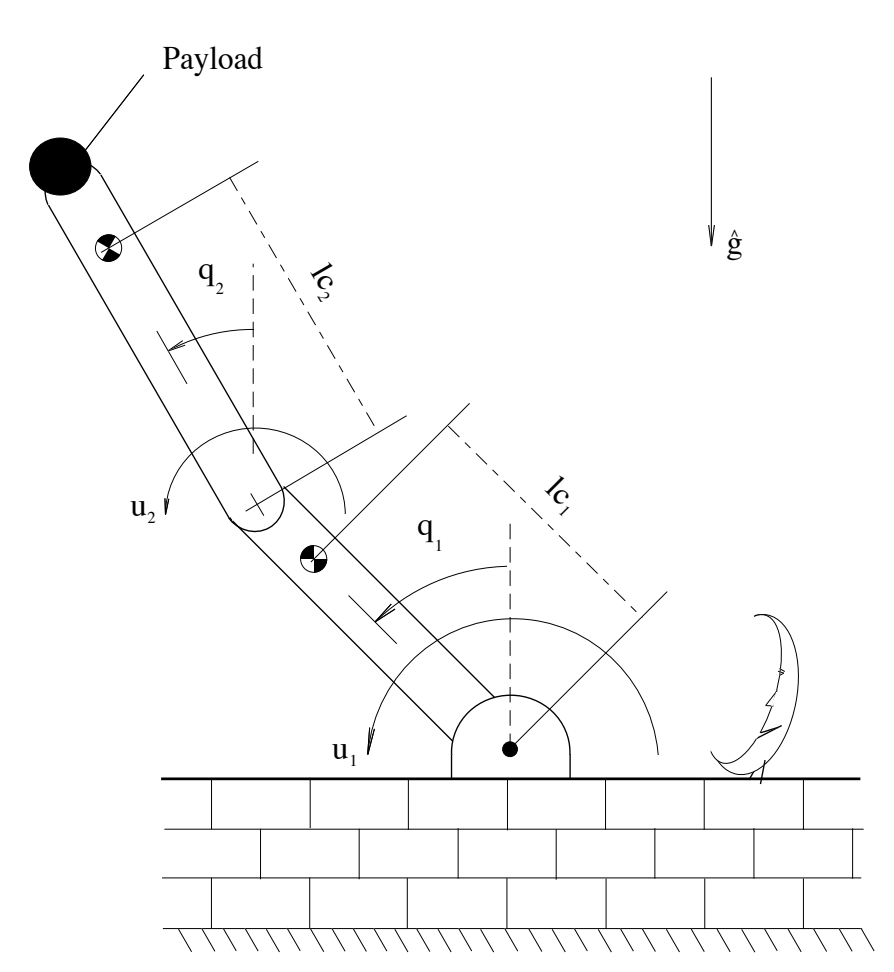
\includegraphics[width=.24\linewidth]{figures/manipulator.png}\end{center}
\end{questionprompt}
\subsection*{Solution}
% 在這裡撰寫解答。
\vspace{3.5cm}


\begin{questionprompt}
\section*{Exercise 34}
\phantomsection\label{practice:34}
{\small Source: Exercise 13; textbook pp.~41--42.}\par
Recall the ``two link manipulator'' example in the notes.
\begin{enumerate}[label=(\roman*)]
\item By appropriate definition of state variables, obtain a first order state space description of this system.
\item Find all equilibrium states.
\end{enumerate}
\editorial{練習版本：平衡點問題明定採零輸入 $u=0$（two-link manipulator 為 $u_1=u_2=0$）；Exercise 13 另略去原 (iii) 的 MATLAB 模擬。}

The referenced two-link manipulator is described by
\begin{align*}
m_{11}\ddot q_1+m_{12}\cos(q_1-q_2)\ddot q_2+c_1\sin(q_1-q_2)\dot q_2^2+g_1\sin q_1&=u_1,\\
m_{21}\cos(q_1-q_2)\ddot q_1+m_{22}\ddot q_2+c_2\sin(q_1-q_2)\dot q_1^2+g_2\sin q_2&=u_2,
\end{align*}
where
\begin{align*}
m_{11}&=I_1+m_1l_{c1}^2+m_2l_1^2,& m_{12}=m_{21}&=m_2l_1l_{c2},\\
m_{22}&=I_2+m_2l_{c2}^2,&g_1&=-(m_1l_{c1}+m_2l_1)g,\\
g_2&=-m_2l_{c2}g,&c_1=-c_2&=m_2l_1l_{c2}.
\end{align*}
Here $q_1,q_2$ are link angles relative to the local vertical.
\begin{center}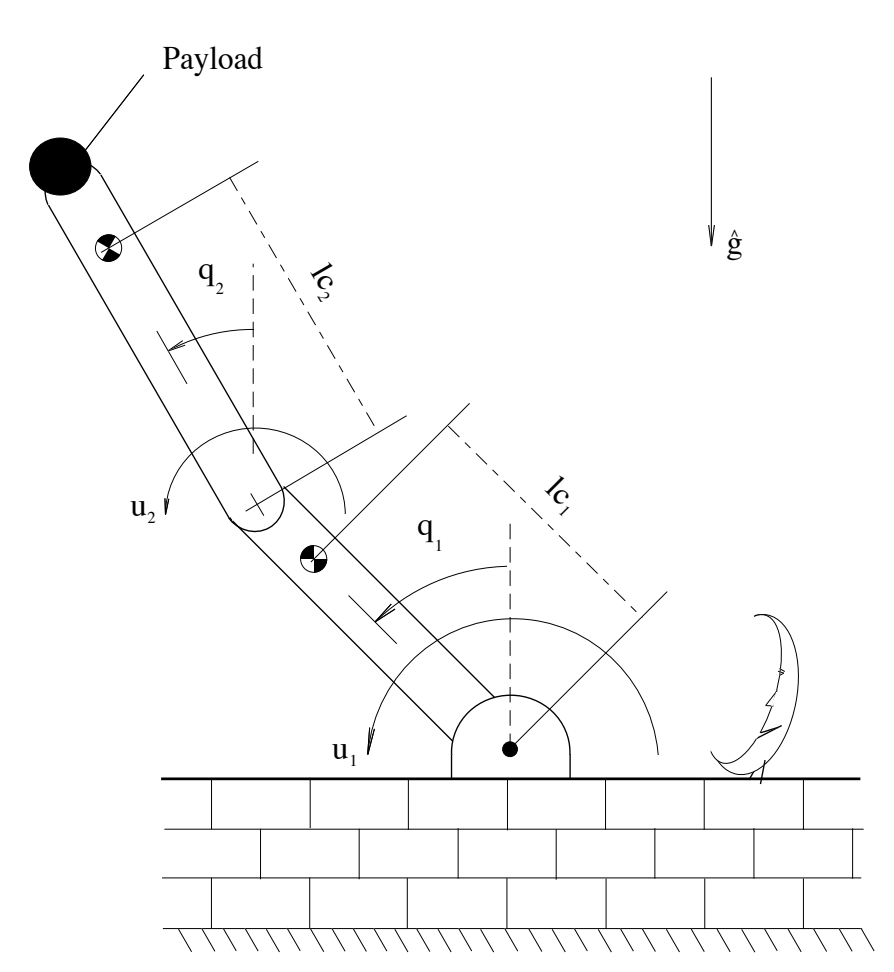
\includegraphics[width=.32\linewidth]{figures/manipulator.png}\end{center}
\end{questionprompt}
\subsection*{Solution}
% 在這裡撰寫解答。
\vspace{3.5cm}


\begin{questionprompt}
\section*{Exercise 35}
\phantomsection\label{practice:35}
{\small Source: Exercise 4; textbook pp.~25--26.}\par
By appropriate definition of state variables, obtain a first order state space description of the following systems, where $q_1,q_2$ are real scalars.
\begin{enumerate}[label=(\roman*)]
\item $2\ddot q_1+3\ddot q_2+\dot q_1-q_2=0,\quad \ddot q_1+2\ddot q_2-\dot q_2+q_1=0$.
\item $q_2^{(3)}+2\dot q_1+q_2-q_1=0,\quad \ddot q_2+\dot q_1-q_2+q_1=0$.
\end{enumerate}
\end{questionprompt}
\subsection*{Solution}
% 在這裡撰寫解答。
\vspace{3.5cm}


\begin{questionprompt}
\section*{Exercise 36}
\phantomsection\label{practice:36}
{\small Source: Exercise 80; textbook pp.~163.}\par
Compute expressions for eigenvalues and linearly independent eigenvectors of
\[A=\begin{bmatrix}\alpha&\omega\\-\omega&\alpha\end{bmatrix},\qquad\alpha,\omega\ne0.\]
\end{questionprompt}
\subsection*{Solution}
% 在這裡撰寫解答。
\vspace{3.5cm}


\begin{questionprompt}
\section*{Exercise 37}
\phantomsection\label{practice:37}
{\small Source: Exercise 78; textbook pp.~163.}\par
Compute the eigenvalues and eigenvectors of the matrix
\[A=\begin{bmatrix}1&1&0\\0&2&1\\0&0&3\end{bmatrix}.\]
\editorial{數值調整版：改用較小整數的三階矩陣，保留三個互異實特徵值與完整特徵向量組的計算。}
\end{questionprompt}
\subsection*{Solution}
% 在這裡撰寫解答。
\vspace{3.5cm}


\begin{questionprompt}
\section*{Exercise 38}
\phantomsection\label{practice:38}
{\small Source: Exercise 14; textbook pp.~42.}\par
Recall the two pendulum cart example in the notes.
\begin{enumerate}[label=(\alph*)]
\item Obtain all equilibrium configurations corresponding to $u=0$.
\end{enumerate}
\editorial{略去原 (b) 的全部數值模擬要求及其專用參數、初值。}

The double pendulum on a cart has cart displacement $y$, pendulum angles
$\theta_1,\theta_2$, and applied cart force $u$:
\begin{align*}
&(m_0+m_1+m_2)\ddot y-m_1l_1\cos\theta_1\ddot\theta_1-m_2l_2\cos\theta_2\ddot\theta_2\\
&\hspace{15mm}+m_1l_1\sin\theta_1\dot\theta_1^2+m_2l_2\sin\theta_2\dot\theta_2^2=u,\\
&-m_1l_1\cos\theta_1\ddot y+m_1l_1^2\ddot\theta_1+m_1l_1g\sin\theta_1=0,\\
&-m_2l_2\cos\theta_2\ddot y+m_2l_2^2\ddot\theta_2+m_2l_2g\sin\theta_2=0.
\end{align*}
\begin{center}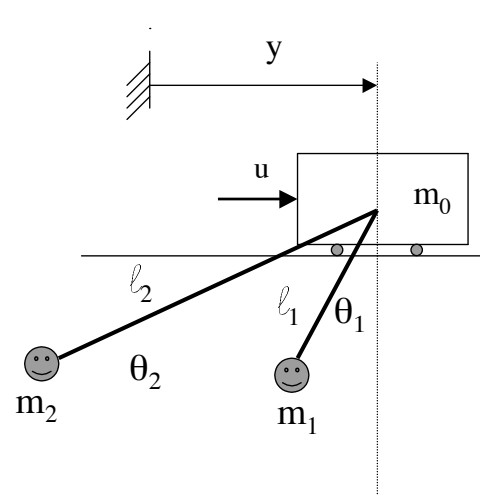
\includegraphics[width=.4\linewidth]{figures/pendulum_cart.png}\end{center}
\end{questionprompt}
\subsection*{Solution}
% 在這裡撰寫解答。
\vspace{3.5cm}


\begin{questionprompt}
\section*{Exercise 39}
\phantomsection\label{practice:39}
{\small Source: Exercise 36; textbook pp.~88.}\par
Obtain a state space realization of the transfer function
\[\widehat G(s)=\begin{bmatrix}\dfrac{1}{s-1}&\dfrac{1}{s-1}\\[5pt]\dfrac{1}{s+1}&-\dfrac{1}{s+1}\end{bmatrix}.\]
\end{questionprompt}
\subsection*{Solution}
% 在這裡撰寫解答。
\vspace{3.5cm}


\begin{questionprompt}
\section*{Exercise 40}
\phantomsection\label{practice:40}
{\small Source: Exercise 40; textbook pp.~88.}\par
\begin{enumerate}[label=(\alph*)]
\item Obtain a state space realization of the following single-input single-output system:
\[\ddot y-3\dot y-4y=\ddot u-2\dot u-8u.\]
\item Is your realization minimal?
\end{enumerate}
\end{questionprompt}
\subsection*{Solution}
% 在這裡撰寫解答。
\vspace{3.5cm}


\begin{questionprompt}
\section*{Exercise 41}
\phantomsection\label{practice:41}
{\small Source: Exercise 93; textbook pp.~184.}\par
Suppose $A$ is a $3\times3$ matrix, $b$ is a $3$-vector, and
\[\det(sI-A)=s^3+2s^2+s+1.\]
\begin{enumerate}[label=(\alph*)]
\item Express $A^3b$ in terms of $b,Ab,A^2b$.
\item Suppose $T=\begin{bmatrix}b&Ab&A^2b\end{bmatrix}$ is invertible. What is $\Lambda:=T^{-1}AT$? Specify each element explicitly.
\end{enumerate}
\end{questionprompt}
\subsection*{Solution}
% 在這裡撰寫解答。
\vspace{3.5cm}


\begin{questionprompt}
\section*{Exercise 42}
\phantomsection\label{practice:42}
{\small Source: Exercise 85; textbook pp.~165.}\par
Suppose $A$ is a real square matrix with characteristic polynomial
\[p(s)=(s+2)(s^2+4)^2.\]
Suppose that all eigenvectors of $A$ are nonzero multiples of
\[\begin{bmatrix}1\\2\\3\\4\\0\end{bmatrix},\quad
\begin{bmatrix}0\\1+j\\-j\\0\\1\end{bmatrix},\quad\text{or}\quad
\begin{bmatrix}0\\1-j\\j\\0\\1\end{bmatrix}.\]
For this practice version, the three displayed vectors correspond, in order, to eigenvalues $-2,2j,-2j$. What is the solution of $\dot x=Ax$ with these initial conditions?
\[(a)\ \begin{bmatrix}2\\4\\6\\8\\0\end{bmatrix}\quad
(b)\ \begin{bmatrix}0\\1\\0\\0\\1\end{bmatrix}\quad
(c)\ \begin{bmatrix}0\\0\\1\\0\\1\end{bmatrix}.\]
(d) Are all solutions of $\dot x=Ax$ bounded? Justify your answer.
\editorial{練習版本：本卷已明定各向量與特徵值的對應，原書未逐一標示。}
\end{questionprompt}
\subsection*{Solution}
% 在這裡撰寫解答。
\vspace{3.5cm}


\begin{questionprompt}
\section*{Exercise 43}
\phantomsection\label{practice:43}
{\small Source: Exercise 71; textbook pp.~141.}\par
Consider the delay differential equation
\[\dot x(t)=A_1x(t)+A_2x(t-1),\qquad t\in\mathbb R,\quad x(t)\in\mathbb C^n.\]
Show that if a complex number $\lambda$ satisfies
\[\det(\lambda I-A_1-e^{-\lambda}A_2)=0,\]
then the delay differential equation has a solution of the form $e^{\lambda t}v$, where $v\in\mathbb C^n$ is nonzero.
\end{questionprompt}
\subsection*{Solution}
% 在這裡撰寫解答。
\vspace{3.5cm}


\begin{questionprompt}
\section*{Exercise 44}
\phantomsection\label{practice:44}
{\small Source: Exercise 58; textbook pp.~110.}\par
\begin{enumerate}[label=(\alph*)]\item Find a basis for the range of the matrix
\[A=\begin{bmatrix}1&2&3&4\\2&3&4&5\\3&4&5&6\end{bmatrix}.\]
\item What is the rank of $A$?\end{enumerate}
\editorial{略去 MATLAB 核對要求。}
\end{questionprompt}
\subsection*{Solution}
% 在這裡撰寫解答。
\vspace{3.5cm}


\begin{questionprompt}
\section*{Exercise 45}
\phantomsection\label{practice:45}
{\small Source: Exercise 54; textbook pp.~102.}\par
Consider $m$ vectors $x^{(1)},\ldots,x^{(m)}\in\mathbb R^n$, $m\le n$, with the following structure: the first $n_i-1$ components of the $i$th vector are zero, its $n_i$th component is nonzero, and
\[1\le n_1<n_2<\cdots<n_m\le n.\]
Prove that this collection is linearly independent.
\editorial{以原書緊接向量圖後的文字條件排寫；原文索引 $n_{nm}$ 明確按第 $m$ 個首個非零位置 $n_m$ 排寫。}
\end{questionprompt}
\subsection*{Solution}
% 在這裡撰寫解答。
\vspace{3.5cm}


\begin{questionprompt}
\section*{Exercise 46}
\phantomsection\label{practice:46}
{\small Source: Exercise 59; textbook pp.~111.}\par
Obtain a basis for the range of each of the following matrices. Also, what is the rank and nullity of each matrix?
\[A_1=\begin{bmatrix}1&0&1\\0&1&1\\1&1&1\end{bmatrix},\qquad
A_2=\begin{bmatrix}0&1&0\\0&0&0\\0&0&1\end{bmatrix},\qquad
A_3=\begin{bmatrix}1&0&1&2&0\\0&1&1&0&2\\1&1&1&1&1\end{bmatrix}.\]\editorial{數值調整版：原第一、第三個矩陣改為較小整數且保留值域、秩與零空間練習；第二個矩陣保留。略去 MATLAB 核對。}
\end{questionprompt}
\subsection*{Solution}
% 在這裡撰寫解答。
\vspace{3.5cm}


\begin{questionprompt}
\section*{Exercise 47}
\phantomsection\label{practice:47}
{\small Source: Exercise 79; textbook pp.~163.}\par
Compute the eigenvalues and eigenvectors of the matrix
\[A=\begin{bmatrix}0&1&0&0\\0&0&1&0\\0&0&0&1\\1&0&0&0\end{bmatrix}.\]
\end{questionprompt}
\subsection*{Solution}
% 在這裡撰寫解答。
\vspace{3.5cm}


\begin{questionprompt}
\section*{Exercise 48}
\phantomsection\label{practice:48}
{\small Source: Exercise 41; textbook pp.~88.}\par
Obtain a state space realization of the following input-output system.
\[\ddot y_1-y_1+y_2=\dot u_1+u_1,\qquad\ddot y_2+y_2-y_1=u_2.\]
\end{questionprompt}
\subsection*{Solution}
% 在這裡撰寫解答。
\vspace{3.5cm}


\begin{questionprompt}
\section*{Exercise 49}
\phantomsection\label{practice:49}
{\small Source: Exercise 37; textbook pp.~88.}\par
Obtain a state space realization of the transfer function
\[\widehat G(s)=\begin{bmatrix}\dfrac{s}{s-1}&\dfrac{1}{s+1}\end{bmatrix}.\]
Is your realization minimal?
\end{questionprompt}
\subsection*{Solution}
% 在這裡撰寫解答。
\vspace{3.5cm}


\begin{questionprompt}
\section*{Exercise 50}
\phantomsection\label{practice:50}
{\small Source: Exercise 31; textbook pp.~71.}\par
Obtain the transfer function of the following system:
\[\dot x(t)=-x(t)+2x(t-h)+u(t),\qquad y(t)=x(t).\]
\end{questionprompt}
\subsection*{Solution}
% 在這裡撰寫解答。
\vspace{3.5cm}


\begin{questionprompt}
\section*{Exercise 51}
\phantomsection\label{practice:51}
{\small Source: Exercise 102; textbook pp.~185.}\par
Suppose
\[A=\begin{bmatrix}0&1&0&0\\0&0&1&0\\0&0&0&1\\0&0&0&0\end{bmatrix}.\]
What is $A^{20}+4A^4$?
\end{questionprompt}
\subsection*{Solution}
% 在這裡撰寫解答。
\vspace{3.5cm}


\begin{questionprompt}
\section*{Exercise 52}
\phantomsection\label{practice:52}
{\small Source: Unnumbered R(A); textbook pp.~108.}\par
For a real $m\times n$ matrix $A$, define
\[\mathcal R(A)=\{Ax:x\in\mathbb R^n\}.\]
Show that $\mathcal R(A)$ is a subspace of $\mathbb R^m$.
\editorial{原書正文標示為 Exercise 的未編號練習。}
\end{questionprompt}
\subsection*{Solution}
% 在這裡撰寫解答。
\vspace{3.5cm}


\begin{questionprompt}
\section*{Exercise 53}
\phantomsection\label{practice:53}
{\small Source: Exercise 27; textbook pp.~60--61.}\par
(Simple pendulum in drag.) Recall the simple pendulum in drag whose motion is described by
\[ml\ddot\theta+\kappa V(l\dot\theta-w\sin\theta)+mg\sin\theta=0,\]
where
\[V=\sqrt{l^2\dot\theta^2+w^2-2lw\sin(\theta)\dot\theta},\qquad\kappa=\frac{\rho SC_D}{2}.\]
Here $g$ is gravitational acceleration, $S$ is the reference area associated with the ball, $C_D$ is its drag coefficient, and $\rho$ is air density.
\editorial{原 PDF 的 Figure 3.1 僅有圖說、圖像為空白；此處保留完整運動方程式。}
\begin{enumerate}[label=(\alph*)]
\item Obtain the equilibrium values $\theta_e$ of $\theta$.
\item Linearize the system about $\theta_e$.
\item Obtain an expression for the $A$ matrix for a state space representation of the linearized system.
\end{enumerate}
\editorial{略去原 (d) 的非線性／線性數值比較、時間圖與專用參數。}
\end{questionprompt}
\subsection*{Solution}
% 在這裡撰寫解答。
\vspace{3.5cm}


\begin{questionprompt}
\section*{Exercise 54}
\phantomsection\label{practice:54}
{\small Source: Exercise 10; textbook pp.~41.}\par
Obtain a state-space description of the following system.
\[q_1^{(3)}+\dot q_2+q_1=0,\qquad \ddot q_1-\dot q_2+q_2=0.\]
\end{questionprompt}
\subsection*{Solution}
% 在這裡撰寫解答。
\vspace{3.5cm}


\begin{questionprompt}
\section*{Exercise 55}
\phantomsection\label{practice:55}
{\small Source: Exercise 81; textbook pp.~163.}\par
Find expressions for the eigenvalues and linearly independent eigenvectors of matrices of the form
\[\begin{bmatrix}\beta&\gamma\\\gamma&\beta\end{bmatrix},\qquad\beta,\gamma\in\mathbb R,\quad\gamma\ge0.\]
\editorial{略去原題要求的三組 state plane portraits，不需畫相圖。}
\end{questionprompt}
\subsection*{Solution}
% 在這裡撰寫解答。
\vspace{3.5cm}


\begin{questionprompt}
\section*{Exercise 56}
\phantomsection\label{practice:56}
{\small Source: Exercise 43; textbook pp.~89.}\par
Obtain a state space realization of the following input-output system.
\[\dot y_1+y_2=\dot u_2+u_1,\qquad\dot y_2+y_1=\dot u_1+u_2.\]
\end{questionprompt}
\subsection*{Solution}
% 在這裡撰寫解答。
\vspace{3.5cm}


\begin{questionprompt}
\section*{Exercise 57}
\phantomsection\label{practice:57}
{\small Source: Exercise 57; textbook pp.~110.}\par
\begin{enumerate}[label=(\alph*)]\item Find a basis for the null space of the matrix
\[A=\begin{bmatrix}1&2&3&4\\2&3&4&5\\3&4&5&6\end{bmatrix}.\]
\item What is the nullity of $A$?\end{enumerate}
\editorial{略去 MATLAB 核對要求。}
\end{questionprompt}
\subsection*{Solution}
% 在這裡撰寫解答。
\vspace{3.5cm}


\begin{questionprompt}
\section*{Exercise 58}
\phantomsection\label{practice:58}
{\small Source: Exercise 26; textbook pp.~60.}\par
\begin{enumerate}[label=(\alph*)]
\item Obtain all equilibrium solutions of the following system:
\begin{align*}
(\cos q_1)\ddot q_1+(\sin q_1)\ddot q_2+(\sin q_2)\dot q_1^2+\sin q_2&=0,\\
-(\sin q_1)\ddot q_1+(\cos q_1)\ddot q_2+(\cos q_2)\dot q_2^2+\sin q_1&=0.
\end{align*}
\item Linearize the above system about its zero solution.
\end{enumerate}
\end{questionprompt}
\subsection*{Solution}
% 在這裡撰寫解答。
\vspace{3.5cm}


\begin{questionprompt}
\section*{Exercise 59}
\phantomsection\label{practice:59}
{\small Source: Exercise 6; textbook pp.~26.}\par
Obtain a state-space description of the following single-input single-output system with input $u$ and output $y$.
\[\ddot q_1+\dot q_2+q_1=0,\qquad \ddot q_1-\dot q_2+q_2=u,\qquad y=\ddot q_1.\]
\end{questionprompt}
\subsection*{Solution}
% 在這裡撰寫解答。
\vspace{3.5cm}


\begin{questionprompt}
\section*{Exercise 60}
\phantomsection\label{practice:60}
{\small Source: Exercise 18; textbook pp.~46.}\par
Determine which of the following matrices are invertible, and determine the inverse of those that are invertible.
\[(a)\ \begin{bmatrix}1&1&0\\0&0&1\\1&0&0\end{bmatrix}\quad
(b)\ \begin{bmatrix}1&0&1\\1&0&1\\1&0&1\end{bmatrix}\quad
(c)\ \begin{bmatrix}0&1&0\\1&0&1\\0&1&0\end{bmatrix}.\]
\editorial{將原本以 MATLAB 求逆及核對改為手算。}
\end{questionprompt}
\subsection*{Solution}
% 在這裡撰寫解答。
\vspace{3.5cm}


\begin{questionprompt}
\section*{Exercise 61}
\phantomsection\label{practice:61}
{\small Source: Exercise 46; textbook pp.~96.}\par
Determine whether or not the following system of linear equations has a solution. If a solution exists, determine whether or not it is unique; if not unique, obtain an expression for all solutions.
\begin{align*}x_1-x_2+2x_3+x_4&=5\\x_1-x_2+x_3&=3\\-2x_1+2x_2+2x_4&=-2\\2x_1-2x_2-x_3-3x_4&=0\end{align*}
\end{questionprompt}
\subsection*{Solution}
% 在這裡撰寫解答。
\vspace{3.5cm}


\begin{questionprompt}
\section*{Exercise 62}
\phantomsection\label{practice:62}
{\small Source: Exercise 38; textbook pp.~88.}\par
Obtain a state space realization of the transfer function
\[\widehat G(s)=\begin{bmatrix}\dfrac{s^2+1}{s^2-1}&\dfrac{2}{s-1}\end{bmatrix}.\]
\end{questionprompt}
\subsection*{Solution}
% 在這裡撰寫解答。
\vspace{3.5cm}


\begin{questionprompt}
\section*{Exercise 63}
\phantomsection\label{practice:63}
{\small Source: Exercise 101; textbook pp.~185.}\par
Suppose $A$ is a $4\times4$ matrix with four distinct eigenvalues $-1,1,-j,j$. Show that $A^4=I$.
\editorial{原書在 $+1$ 與 $-j$ 間缺逗號，且未明列矩陣階數。本題為明確化的練習版本：採四階矩陣與上述四個互異特徵值。}
\end{questionprompt}
\subsection*{Solution}
% 在這裡撰寫解答。
\vspace{3.5cm}


\begin{questionprompt}
\section*{Exercise 64}
\phantomsection\label{practice:64}
{\small Source: Exercise 106; textbook pp.~186.}\par
Compute $e^{At}$ at $t=\ln2$ for
\[A=\begin{bmatrix}0&1\\-1&0\end{bmatrix}\]
using Jordan form and the Laplace transform.
\editorial{原題要求筆記的四種方法；略去 MATLAB 與數值模擬。}
\end{questionprompt}
\subsection*{Solution}
% 在這裡撰寫解答。
\vspace{3.5cm}


\begin{questionprompt}
\section*{Exercise 65}
\phantomsection\label{practice:65}
{\small Source: Exercise 50; textbook pp.~97.}\par
Determine whether or not the following system of linear equations has a solution. If a solution exists, determine whether or not it is unique; if not unique, obtain an expression for all solutions and give two solutions.
\begin{align*}x_1-2x_2-4x_3&=-1\\2x_1-3x_2-5x_3&=-1\\x_1+2x_3&=1\\x_1+x_2+5x_3&=2\end{align*}
\end{questionprompt}
\subsection*{Solution}
% 在這裡撰寫解答。
\vspace{3.5cm}


\begin{questionprompt}
\section*{Exercise 66}
\phantomsection\label{practice:66}
{\small Source: Exercise 2; textbook pp.~25.}\par
By appropriate definition of state variables, obtain a first order state space description of the following systems.
\begin{enumerate}[label=(\roman*)]
\item The ``simple structure'' (Section 2.1.4, p.~9):
\begin{align*}
m_1\ddot q_1+(c_1+c_2)\dot q_1+(k_1+k_2)q_1-c_2\dot q_2-k_2q_2&=u_1,\\
m_2\ddot q_2-c_2\dot q_1-k_2q_1+c_2\dot q_2+k_2q_2&=u_2.
\end{align*}
\item The ``body in central force motion'' (Section 2.2.4, p.~12):
\[\ddot r-r\omega^2+g(r)=0,\qquad r\dot\omega+2\dot r\omega=0.\]
Here $r$ is radial distance and $\omega$ is angular rate.
\item $q_1,q_2$ are real scalars:
\[\ddot q_1+q_1+2\dot q_2=0,\qquad \ddot q_1+\dot q_2+q_2=0.\]
\end{enumerate}
\end{questionprompt}
\subsection*{Solution}
% 在這裡撰寫解答。
\vspace{3.5cm}


\begin{questionprompt}
\section*{Exercise 67}
\phantomsection\label{practice:67}
{\small Source: Exercise 39; textbook pp.~88.}\par
Obtain a state space representation of the following input-output system.
\[2\frac{d^3y}{dt^3}+6\frac{d^2y}{dt^2}+4\frac{dy}{dt}+2y
=6\frac{d^2u}{dt^2}+10\frac{du}{dt}+8u.\]
\end{questionprompt}
\subsection*{Solution}
% 在這裡撰寫解答。
\vspace{3.5cm}


\begin{questionprompt}
\section*{Exercise 68}
\phantomsection\label{practice:68}
{\small Source: Exercise 98; textbook pp.~185.}\par
Compute $e^{At}$ for the matrix $A=\begin{bmatrix}3&-5\\-5&3\end{bmatrix}$.
\end{questionprompt}
\subsection*{Solution}
% 在這裡撰寫解答。
\vspace{3.5cm}


\begin{questionprompt}
\section*{Exercise 69}
\phantomsection\label{practice:69}
{\small Source: Exercise 87; textbook pp.~166.}\par
Determine whether or not the following matrix is nondefective.
\[A=\begin{bmatrix}0&1&0\\0&0&1\\-1&1&1\end{bmatrix}.\]
\end{questionprompt}
\subsection*{Solution}
% 在這裡撰寫解答。
\vspace{3.5cm}


\begin{questionprompt}
\section*{Exercise 70}
\phantomsection\label{practice:70}
{\small Source: Exercise 60; textbook pp.~111.}\par
Obtain a basis for the null space of each of the following matrices (the same matrices used in the adapted Exercise 59).
\[A_1=\begin{bmatrix}1&0&1\\0&1&1\\1&1&1\end{bmatrix},\qquad
A_2=\begin{bmatrix}0&1&0\\0&0&0\\0&0&1\end{bmatrix},\qquad
A_3=\begin{bmatrix}1&0&1&2&0\\0&1&1&0&2\\1&1&1&1&1\end{bmatrix}.\]\editorial{數值調整版：與本卷原 Exercise 59 同步。略去 MATLAB 核對，並直接重列矩陣，方便打散後獨立作答。}
\end{questionprompt}
\subsection*{Solution}
% 在這裡撰寫解答。
\vspace{3.5cm}


\begin{questionprompt}
\section*{Exercise 71}
\phantomsection\label{practice:71}
{\small Source: Exercise 94; textbook pp.~184.}\par
Suppose $A$ is a $3\times3$ matrix and
\[\det(sI-A)=s^3+2s^2+s+1.\]
\begin{enumerate}[label=(\alph*)]
\item Express $A^3$ in terms of $I,A,A^2$.
\item Express $A^5$ in terms of $I,A,A^2$.
\item Express $A^{-1}$ in terms of $I,A,A^2$.
\end{enumerate}
\end{questionprompt}
\subsection*{Solution}
% 在這裡撰寫解答。
\vspace{3.5cm}


\begin{questionprompt}
\section*{Exercise 72}
\phantomsection\label{practice:72}
{\small Source: Exercise 95; textbook pp.~184.}\par
Suppose $A$ is a $3\times3$ matrix with eigenvalues $1,2\pi j,-2\pi j$. What are the eigenvalues of $e^A$?
\end{questionprompt}
\subsection*{Solution}
% 在這裡撰寫解答。
\vspace{3.5cm}


\begin{questionprompt}
\section*{Exercise 73}
\phantomsection\label{practice:73}
{\small Source: Exercise 103; textbook pp.~185.}\par
Suppose $A$ is a $3\times3$ matrix with eigenvalues $1,2\pi j,-2\pi j$. What are the eigenvalues of $e^A$?
\end{questionprompt}
\subsection*{Solution}
% 在這裡撰寫解答。
\vspace{3.5cm}


\begin{questionprompt}
\section*{Exercise 74}
\phantomsection\label{practice:74}
{\small Source: Exercise 28; textbook pp.~66.}\par
Show that the transfer function of
\[\dot x_1=x_2,\quad\dot x_2=-\alpha_0x_1-\alpha_1x_2+u,\quad y=\beta_0x_1+\beta_1x_2\]
is given by
\[\widehat G(s)=\frac{\beta_1s+\beta_0}{s^2+\alpha_1s+\alpha_0}.\]
\end{questionprompt}
\subsection*{Solution}
% 在這裡撰寫解答。
\vspace{3.5cm}


\begin{questionprompt}
\section*{Exercise 75}
\phantomsection\label{practice:75}
{\small Source: Exercise 99; textbook pp.~185.}\par
Compute $e^{At}$ for the matrix $A=\begin{bmatrix}-3&4\\-2&3\end{bmatrix}$.
\editorial{數值調整版：原矩陣 $\left[\begin{smallmatrix}-11&20\\-6&11\end{smallmatrix}\right]$ 改用較小整數；保留非對稱矩陣與正負實模態。}
\end{questionprompt}
\subsection*{Solution}
% 在這裡撰寫解答。
\vspace{3.5cm}


\begin{questionprompt}
\section*{Exercise 76}
\phantomsection\label{practice:76}
{\small Source: Exercise 52; textbook pp.~97.}\par
We consider systems of linear equations $Ax=b$ with $x=(x_1,x_2,x_3)^T$.
For each case, the reduced row echelon form of the augmented matrix $[A\ b]$ is given below. Determine whether or not the system has a solution. If a solution exists, determine whether or not it is unique; if not unique, obtain an expression for all solutions and give two solutions.
\begin{align*}
(a)&\ \begin{bmatrix}1&5&0&0\\0&0&1&0\\0&0&0&1\end{bmatrix},&
(b)&\ \begin{bmatrix}1&-2&0&6\\0&0&1&4\\0&0&0&0\end{bmatrix},\\
(c)&\ \begin{bmatrix}1&2&0&0\\0&0&1&0\\0&0&0&1\\0&0&0&0\end{bmatrix},&
(d)&\ \begin{bmatrix}1&0&0&0\\0&1&0&0\\0&0&1&0\\0&0&0&1\end{bmatrix}.
\end{align*}
\end{questionprompt}
\subsection*{Solution}
% 在這裡撰寫解答。
\vspace{3.5cm}


\begin{questionprompt}
\section*{Exercise 77}
\phantomsection\label{practice:77}
{\small Source: Exercise 104; textbook pp.~186.}\par
Compute $e^{At}$ for the matrix $A=\begin{bmatrix}-3&2\\-4&3\end{bmatrix}$.
\end{questionprompt}
\subsection*{Solution}
% 在這裡撰寫解答。
\vspace{3.5cm}


\begin{questionprompt}
\section*{Exercise 78}
\phantomsection\label{practice:78}
{\small Source: Exercise 97; textbook pp.~185.}\par
Suppose $A$ is a square matrix.
\begin{enumerate}[label=(\alph*)]
\item Obtain expressions for $\cos(At)$ and $\sin(At)$.
\item Show that
\[\cos(At)=\frac{e^{jAt}+e^{-jAt}}{2},\qquad
\sin(At)=\frac{e^{jAt}-e^{-jAt}}{2j}.\]
\item Show that
\[\frac{d\cos(At)}{dt}=-A\sin(At),\qquad\frac{d\sin(At)}{dt}=A\cos(At).\]
\end{enumerate}
\end{questionprompt}
\subsection*{Solution}
% 在這裡撰寫解答。
\vspace{3.5cm}


\begin{questionprompt}
\section*{Exercise 79}
\phantomsection\label{practice:79}
{\small Source: Exercise 68; textbook pp.~130.}\par
What is the companion matrix whose eigenvalues are $-1,-2,-3$?
\end{questionprompt}
\subsection*{Solution}
% 在這裡撰寫解答。
\vspace{3.5cm}


\begin{questionprompt}
\section*{Exercise 80}
\phantomsection\label{practice:80}
{\small Source: Exercise 49; textbook pp.~97.}\par
Determine whether or not the following system of linear equations has a solution. If a solution exists, determine whether or not it is unique; if not unique, obtain an expression for all solutions and give two solutions.
\begin{align*}x_2+x_4&=2\\2x_1+3x_2+2x_3+3x_4&=8\\x_1+x_2+x_3+x_4&=3\end{align*}
\end{questionprompt}
\subsection*{Solution}
% 在這裡撰寫解答。
\vspace{3.5cm}


\begin{questionprompt}
\section*{Exercise 81}
\phantomsection\label{practice:81}
{\small Source: Exercise 44; textbook pp.~89.}\par
Consider the single-input single-output system described by
\[\dot x_1=-2x_2+u,\qquad\dot x_2=-2x_1+u,\qquad y=x_1-x_2.\]
\begin{enumerate}[label=(\alph*)]
\item Compute $e^{At}$ for $A=\begin{bmatrix}0&-2\\-2&0\end{bmatrix}$.
\item Obtain the impulse response of the system.
\item What is the transfer function of this system?
\end{enumerate}
\end{questionprompt}
\subsection*{Solution}
% 在這裡撰寫解答。
\vspace{3.5cm}


\begin{questionprompt}
\section*{Exercise 82}
\phantomsection\label{practice:82}
{\small Source: Exercise 74; textbook pp.~149--150.}\par
Show that if $A$ is similar to $\Lambda$, then:
\begin{enumerate}[label=(\alph*)]
\item $\det A=\det\Lambda$.
\item $\operatorname{charpoly}A=\operatorname{charpoly}\Lambda$ and hence $A$ and $\Lambda$ have the same eigenvalues with the same algebraic multiplicities.
\end{enumerate}
\end{questionprompt}
\subsection*{Solution}
% 在這裡撰寫解答。
\vspace{3.5cm}


\begin{questionprompt}
\section*{Exercise 83}
\phantomsection\label{practice:83}
{\small Source: Exercise 5; textbook pp.~26.}\par
By appropriate definition of state variables, obtain a first order state space description of the following systems, where $q_1,q_2$ are real scalars.
\begin{enumerate}[label=(\roman*)]
\item $3\ddot q_1-\ddot q_2+2\dot q_1+4q_2=0,\quad -\ddot q_1+3\ddot q_2+2\dot q_1-4q_2=0$.
\item $3\ddot q_1-\dot q_2+4q_2-4q_1=0,\quad -\ddot q_1+3\dot q_2-4q_2+4q_1=0$.
\end{enumerate}
\end{questionprompt}
\subsection*{Solution}
% 在這裡撰寫解答。
\vspace{3.5cm}


\begin{questionprompt}
\section*{Exercise 84}
\phantomsection\label{practice:84}
{\small Source: Exercise 76; textbook pp.~158.}\par
Compute the state transition matrix for the continuous-time system $\dot x=Ax$ corresponding to the $A$ matrix in Example 80:
\[A=\begin{bmatrix}4&-2&-2\\0&2&-2\\0&-2&2\end{bmatrix}.\]
\editorial{直接列出 Example 80 的原矩陣，未附其特徵分解。}
\end{questionprompt}
\subsection*{Solution}
% 在這裡撰寫解答。
\vspace{3.5cm}


\begin{questionprompt}
\section*{Exercise 85}
\phantomsection\label{practice:85}
{\small Source: Exercise 69; textbook pp.~132.}\par
Prove the following statement. Suppose $v_1,\ldots,v_m$ are eigenvectors of $A$ with corresponding eigenvalues $\lambda_1,\ldots,\lambda_m$. Then the solution of $\dot x=Ax$ with initial state
\[x_0=\xi_{10}v_1+\cdots+\xi_{m0}v_m,\]
where $\xi_{10},\ldots,\xi_{m0}$ are scalars, is given by
\[x(t)=\xi_{10}e^{\lambda_1t}v_1+\cdots+\xi_{m0}e^{\lambda_mt}v_m.\]
\end{questionprompt}
\subsection*{Solution}
% 在這裡撰寫解答。
\vspace{3.5cm}


\begin{questionprompt}
\section*{Exercise 86}
\phantomsection\label{practice:86}
{\small Source: Exercise 84; textbook pp.~165.}\par
Suppose $A$ is a real square matrix and the vectors
\[\begin{bmatrix}1\\-1\\1\\-1\end{bmatrix},\quad
\begin{bmatrix}1\\2\\4\\8\end{bmatrix},\quad
\begin{bmatrix}1\\j\\-1\\-j\end{bmatrix}\]
are eigenvectors corresponding to $-1,2,j$, respectively. What is the response of $\dot x=Ax$ to these initial conditions?
\[(a)\ \begin{bmatrix}2\\-2\\2\\-2\end{bmatrix}\quad
(b)\ \begin{bmatrix}-1\\-2\\-4\\-8\end{bmatrix}\quad
(c)\ \begin{bmatrix}0\\3\\3\\9\end{bmatrix}\quad
(d)\ \begin{bmatrix}1\\1\\-1\\-1\end{bmatrix}.\]
\end{questionprompt}
\subsection*{Solution}
% 在這裡撰寫解答。
\vspace{3.5cm}


\begin{questionprompt}
\section*{Exercise 87}
\phantomsection\label{practice:87}
{\small Source: Exercise 29; textbook pp.~66.}\par
Show that the transfer function of
\[\dot x_1=-\alpha_0x_2+\beta_0u,\quad\dot x_2=x_1-\alpha_1x_2+\beta_1u,\quad y=x_2\]
is given by
\[\widehat G(s)=\frac{\beta_1s+\beta_0}{s^2+\alpha_1s+\alpha_0}.\]
\end{questionprompt}
\subsection*{Solution}
% 在這裡撰寫解答。
\vspace{3.5cm}


\begin{questionprompt}
\section*{Exercise 88}
\phantomsection\label{practice:88}
{\small Source: Exercise 21; textbook pp.~48.}\par
Suppose $A$ and $B$ are fixed $n\times n$ matrices and consider the map $L$ from $\mathbb R^{n\times n}$ to $\mathbb R^{n\times n}$ given by
\[L(P)=APB\]
for any $n\times n$ matrix $P$. Show that $L$ is a linear map.
\end{questionprompt}
\subsection*{Solution}
% 在這裡撰寫解答。
\vspace{3.5cm}


\begin{questionprompt}
\section*{Exercise 89}
\phantomsection\label{practice:89}
{\small Source: Exercise 70; textbook pp.~140--141.}\par
(Beavis and Butthead at the laundromat.) Consider
\begin{align*}
m\ddot q_1-m\Omega^2q_1+\frac{k}{2}(q_1-q_2-2l_0)&=0,\\
m\ddot q_2-m\Omega^2q_2-\frac{k}{2}(q_1-q_2-2l_0)&=0,
\end{align*}
with $\omega:=\sqrt{k/m}>\Omega$.
\begin{enumerate}[label=(\alph*)]
\item Obtain the equilibrium values $q_1^e,q_2^e$ of $q_1,q_2$.
\item With $x_1=\delta q_1:=q_1-q_1^e$, $x_2=\delta q_2:=q_2-q_2^e$, $x_3=\dot q_1$, $x_4=\dot q_2$, obtain a state space description $\dot x=Ax$.
\item Obtain expressions for the eigenvalues of $A$. Write down the complex Jordan form and real Jordan form of $A$.
\item For the rest of the exercise, consider $\omega^2=2\Omega^2$. Obtain linearly independent eigenvectors of $A$.
\item For $\Omega=1$ and $(\delta q_1(0),\delta q_2(0),\dot q_1(0),\dot q_2(0))=(1,-1,0,0)$, calculate the response. Why is $\delta q_2(t)\equiv-\delta q_1(t)$?
\item With initial data $(1,1,-1,-1)$, calculate the response. Why is $\delta q_2(t)\equiv\delta q_1(t)$? Why does the solution decay to zero?
\item With initial data $(1,1,1,1)$, calculate the response. Why is $\delta q_2(t)\equiv\delta q_1(t)$? Is this solution bounded?
\item With initial data $(1,-1,j,-j)$, calculate the response and $\|x(t)\|$. Is the norm constant? Explain.
\end{enumerate}
\editorial{原 (e)--(h) 的數值模擬與所有圖形改為手算響應；保留原初值與定性問題。}
\end{questionprompt}
\subsection*{Solution}
% 在這裡撰寫解答。
\vspace{3.5cm}


\begin{questionprompt}
\section*{Exercise 90}
\phantomsection\label{practice:90}
{\small Source: Exercise 92; textbook pp.~182.}\par
Compute $e^{At}$ at $t=\ln2$ for
\[A=\begin{bmatrix}0&1\\1&0\end{bmatrix}\]
using the hand-calculation methods in Section 7.5 (Jordan form and Laplace transform).
\editorial{原題要求該節全部方法；略去 MATLAB 與數值模擬。}
\end{questionprompt}
\subsection*{Solution}
% 在這裡撰寫解答。
\vspace{3.5cm}


\begin{questionprompt}
\section*{Exercise 91}
\phantomsection\label{practice:91}
{\small Source: Exercise 25; textbook pp.~59.}\par
For each of the following systems, linearize about each equilibrium solution and obtain the system $A$-matrix for a state space representation of these linearized systems.
\begin{enumerate}[label=(\alph*)]
\item $\ddot q+(q^2-1)\dot q+q=0$, where $q(t)$ is a scalar.
\item $\ddot q+\dot q+q-q^3=0$, where $q(t)$ is a scalar.
\item $q(t),\theta(t)$ are scalars:
\begin{align*}(M+m)\ddot q+ml\ddot\theta\cos\theta-ml\dot\theta^2\sin\theta+kq&=0,\\
ml\ddot q\cos\theta+ml^2\ddot\theta+mgl\sin\theta&=0.
\end{align*}
\item $\ddot q+0.5\dot q|\dot q|+q=0$, where $q(t)$ is a scalar.
\end{enumerate}
\end{questionprompt}
\subsection*{Solution}
% 在這裡撰寫解答。
\vspace{3.5cm}


\begin{questionprompt}
\section*{Exercise 92}
\phantomsection\label{practice:92}
{\small Source: Exercise 62; textbook pp.~122--123.}\par
Suppose $a=\alpha+j\omega$ is genuinely complex and $x=\xi_1+j\xi_2$, where $\alpha,\omega,\xi_1,\xi_2$ are real and $\dot x=ax$. Verify
\[\dot\xi_1=\alpha\xi_1-\omega\xi_2,\qquad\dot\xi_2=\omega\xi_1+\alpha\xi_2.\]
\editorial{將原題 ``Verify the last set of equations'' 所指的前頁條件列出；不附推導。}
\end{questionprompt}
\subsection*{Solution}
% 在這裡撰寫解答。
\vspace{3.5cm}


\begin{questionprompt}
\section*{Exercise 93}
\phantomsection\label{practice:93}
{\small Source: Exercise 34; textbook pp.~88.}\par
Obtain a state space realization of the transfer function
\[\widehat G(s)=\begin{bmatrix}1&\dfrac{1}{s-1}\\[5pt]\dfrac{1}{s+1}&\dfrac{1}{s^2-1}\end{bmatrix}.\]
\end{questionprompt}
\subsection*{Solution}
% 在這裡撰寫解答。
\vspace{3.5cm}


\begin{questionprompt}
\section*{Exercise 94}
\phantomsection\label{practice:94}
{\small Source: Exercise 47; textbook pp.~96.}\par
Determine whether or not the following system of linear equations has a solution. If a solution exists, determine whether or not it is unique; if not unique, obtain an expression for all solutions and give two solutions.
\begin{align*}x_1-2x_2-4x_3&=-1\\2x_1-3x_2-5x_3&=-1\\x_1+2x_3&=1\\x_1+x_2+5x_3&=2\end{align*}
\end{questionprompt}
\subsection*{Solution}
% 在這裡撰寫解答。
\vspace{3.5cm}


\begin{questionprompt}
\section*{Exercise 95}
\phantomsection\label{practice:95}
{\small Source: Exercise 82; textbook pp.~163--164.}\par
Consider an LTI system described by $\dot x=Ax$.
\begin{enumerate}[label=(\alph*)]
\item Suppose the vectors
\[\begin{bmatrix}1\\-1\\1\\-1\end{bmatrix}\quad\text{and}\quad\begin{bmatrix}1\\1\\1\\1\end{bmatrix}\]
are eigenvectors of $A$ corresponding to $-2$ and $3$, respectively. What is the response $x(t)$ to $x(0)=\begin{bmatrix}1\\0\\1\\0\end{bmatrix}$?
\item Suppose $A$ is real and
\[\begin{bmatrix}1\\j\\-1\\-j\end{bmatrix}\]
is an eigenvector corresponding to $2+3j$. What is the response $x(t)$ to $x(0)=\begin{bmatrix}1\\0\\-1\\0\end{bmatrix}$?
\end{enumerate}
\end{questionprompt}
\subsection*{Solution}
% 在這裡撰寫解答。
\vspace{3.5cm}


\begin{questionprompt}
\section*{Exercise 96}
\phantomsection\label{practice:96}
{\small Source: Problem 1; textbook pp.~166--167.}\par
Determine whether or not each of the following matrices is diagonalizable. If not, give a reason. If diagonalizable, obtain an invertible $T$ such that $T^{-1}AT$ is diagonal.
\[(a)\ \begin{bmatrix}0&1&0\\0&0&1\\0&1&0\end{bmatrix}\quad
(b)\ \begin{bmatrix}0&1\\-1&2\end{bmatrix}\quad
(c)\ \begin{bmatrix}1&0&0\\0&0&1\\0&1&0\end{bmatrix}.\]
\end{questionprompt}
\subsection*{Solution}
% 在這裡撰寫解答。
\vspace{3.5cm}


\begin{questionprompt}
\section*{Exercise 97}
\phantomsection\label{practice:97}
{\small Source: Unnumbered N(A); textbook pp.~106.}\par
For a real $m\times n$ matrix $A$, define
\[\mathcal N(A)=\{x\in\mathbb R^n:Ax=0\}.\]
Show that $\mathcal N(A)$ is a subspace of $\mathbb R^n$.
\editorial{原書正文標示為 Exercise 的未編號練習。}
\end{questionprompt}
\subsection*{Solution}
% 在這裡撰寫解答。
\vspace{3.5cm}


\begin{questionprompt}
\section*{Exercise 98}
\phantomsection\label{practice:98}
{\small Source: Exercise 35; textbook pp.~88.}\par
Obtain a state space realization of the transfer function
\[\widehat G(s)=\begin{bmatrix}\dfrac{s+2}{s+1}&\dfrac{1}{s+3}\\[5pt]\dfrac{5}{s+1}&\dfrac{5s+1}{s+2}\end{bmatrix}.\]
\end{questionprompt}
\subsection*{Solution}
% 在這裡撰寫解答。
\vspace{3.5cm}


\begin{questionprompt}
\section*{Exercise 99}
\phantomsection\label{practice:99}
{\small Source: Exercise 8; textbook pp.~26.}\par
Obtain a state space representation of the following system:
\[q(k+n)+a_{n-1}q(k+n-1)+\cdots+a_1q(k+1)+a_0q(k)=0,\]
where $q(k)\in\mathbb R$.
\end{questionprompt}
\subsection*{Solution}
% 在這裡撰寫解答。
\vspace{3.5cm}


\begin{questionprompt}
\section*{Exercise 100}
\phantomsection\label{practice:100}
{\small Source: Exercise 11/12; textbook pp.~41.}\par
\editorial{原書將 Exercise 11 與 Exercise 12 標在同一行，以下三組題目的編號歸屬不明，因此合併保留，不自行重新分配。}
By appropriate definition of state variables, obtain a first order state space description of the following systems where $q_1,q_2$ are real scalars.
\begin{enumerate}[label=(\roman*)]
\item $3\ddot q_1-\ddot q_2+2\dot q_1+4q_2=0,\quad -\ddot q_1+3\ddot q_2+2\dot q_1-4q_2=0$.
\item $3\ddot q_1-\dot q_2+4q_2-4q_1=0,\quad -\ddot q_1+3\dot q_2-4q_2+4q_1=0$.
\end{enumerate}
Obtain a state-space description of the following single-input single-output system with input $u$ and output $y$.
\[\ddot q_1+\dot q_2+q_1=0,\qquad \ddot q_1-\dot q_2+q_2=u,\qquad y=\ddot q_1.\]
Obtain a state-space description of the following system.
\[\ddot q_1+\dot q_2+\sin q_1=u,\qquad \dot q_2+q_1+q_2=0,\qquad y=q_1+q_2.\]
\end{questionprompt}
\subsection*{Solution}
% 在這裡撰寫解答。
\vspace{3.5cm}


\begin{questionprompt}
\section*{Exercise 101}
\phantomsection\label{practice:101}
{\small Source: Exercise 48; textbook pp.~97.}\par
Determine whether or not the following system of linear equations has a solution. If a solution exists, determine whether or not it is unique; if not unique, obtain an expression for all solutions and give two solutions.
\begin{align*}
x_1-2x_2+x_3-2x_4&=-1,\\
-3x_1+7x_2-3x_3+7x_4&=4,\\
2x_1-x_2+2x_3-x_4&=2.
\end{align*}
\editorial{練習版本：原書第一式缺運算符號；本卷明定採加號，其餘係數保留。}
\end{questionprompt}
\subsection*{Solution}
% 在這裡撰寫解答。
\vspace{3.5cm}


\begin{questionprompt}
\section*{Exercise 102}
\phantomsection\label{practice:102}
{\small Source: Exercise 77; textbook pp.~163.}\par
Compute the eigenvalues and eigenvectors of the matrix
\[A=\begin{bmatrix}2&-3&0\\2&-3&0\\3&-5&1\end{bmatrix}.\]
\end{questionprompt}
\subsection*{Solution}
% 在這裡撰寫解答。
\vspace{3.5cm}


\begin{questionprompt}
\section*{Exercise 103}
\phantomsection\label{practice:103}
{\small Source: Exercise 63; textbook pp.~123.}\par
For $\dot\xi_1=\alpha\xi_1-\omega\xi_2$, $\dot\xi_2=\omega\xi_1+\alpha\xi_2$, with $\xi_{10}=\xi_1(0)$ and $\xi_{20}=\xi_2(0)$, verify the following equations:
\begin{align*}
\xi_1(t)&=e^{\alpha t}\cos(\omega t)\xi_{10}-e^{\alpha t}\sin(\omega t)\xi_{20},\\
\xi_2(t)&=e^{\alpha t}\sin(\omega t)\xi_{10}+e^{\alpha t}\cos(\omega t)\xi_{20}.
\end{align*}
\editorial{將原題指涉的待驗證等式列出；略去原書提示。}
\end{questionprompt}
\subsection*{Solution}
% 在這裡撰寫解答。
\vspace{3.5cm}


\begin{questionprompt}
\section*{Exercise 104}
\phantomsection\label{practice:104}
{\small Source: Exercise 17; textbook pp.~46.}\par
Determine which of the following matrices are invertible. Obtain the inverses of those which are.
\[(a)\ \begin{bmatrix}1&1\\0&1\end{bmatrix}\quad
(b)\ \begin{bmatrix}1&1\\1&1\end{bmatrix}\quad
(c)\ \begin{bmatrix}0&1\\0&0\end{bmatrix}\quad
(d)\ \begin{bmatrix}0&1\\1&0\end{bmatrix}.\]
\editorial{略去 MATLAB 核對要求。}
\end{questionprompt}
\subsection*{Solution}
% 在這裡撰寫解答。
\vspace{3.5cm}


\begin{questionprompt}
\section*{Exercise 105}
\phantomsection\label{practice:105}
{\small Source: Exercise 32; textbook pp.~73.}\par
(BB in Laundromat.) Consider
\begin{align*}
m\ddot\phi_1-m\Omega^2\phi_1+\frac{k}{2}(\phi_1-\phi_2)&=b_1u,\\
m\ddot\phi_2-m\Omega^2\phi_2-\frac{k}{2}(\phi_1-\phi_2)&=b_2u,\\
y&=c_1\phi_1+c_2\phi_2.
\end{align*}
For each of the following cases, obtain the system transfer function and its poles; consider $\omega:=\sqrt{k/m}>\Omega$.
\begin{enumerate}[label=(\alph*)]
\item $b_1=1,b_2=0,c_1=1,c_2=0$.
\item (Self excited.) $b_1=1,b_2=-1,c_1=1,c_2=0$.
\item (Mass center measurement.) $b_1=1,b_2=0,c_1=1,c_2=1$.
\item (Self excited and mass center measurement.) $b_1=1,b_2=-1,c_1=1,c_2=1$.
\end{enumerate}
Comment on your results.
\end{questionprompt}
\subsection*{Solution}
% 在這裡撰寫解答。

Let
\[
x = \begin{bmatrix}
	x_1 \\ x_2 \\ x_3
\end{bmatrix} = \begin{bmatrix}
	\phi_1 \\ \phi_2 \\ \dot \phi_1 + \dot \phi_2
\end{bmatrix}
\]


\vspace{3.5cm}


\begin{questionprompt}
\section*{Exercise 106}
\phantomsection\label{practice:106}
{\small Source: Exercise 88; textbook pp.~166.}\par
In vibration analysis, one usually encounters systems described by
\[M\ddot q+Kq=0,\]
where $q(t)$ is an $N$-vector and $M,K$ are square matrices. Suppose $\omega$ is a real number satisfying
\[\det(\omega^2M-K)=0.\]
Show that the system has a solution $q(t)=\sin(\omega t)v$, where $v$ is a constant $N$-vector.
\end{questionprompt}
\subsection*{Solution}
% 在這裡撰寫解答。
\vspace{3.5cm}


\begin{questionprompt}
\section*{Exercise 107}
\phantomsection\label{practice:107}
{\small Source: Exercise 107; textbook pp.~192.}\par
(Optional.) Let $g_k$ be a generalized eigenvector of order $k>1$ for eigenvalue $\lambda$ of $A$, so
\[(A-\lambda I)^kg_k=0,\qquad(A-\lambda I)^{k-1}g_k\ne0.\]
Define $g_i=(A-\lambda I)^{k-i}g_k$ for $i=1,\ldots,k$, and let $G=\{g_1,\ldots,g_k\}$. Show that $G$ is linearly independent.
\editorial{補列原題前文的鏈定義；此題位於第 8 章，列為廣義特徵向量的選做延伸。}
\end{questionprompt}
\subsection*{Solution}
% 在這裡撰寫解答。
\vspace{3.5cm}


\begin{questionprompt}
\section*{Exercise 108}
\phantomsection\label{practice:108}
{\small Source: Exercise 105; textbook pp.~186.}\par
Compute $e^{At}$ for the matrix $A=\begin{bmatrix}3&-5\\-5&3\end{bmatrix}$.
\end{questionprompt}
\subsection*{Solution}
% 在這裡撰寫解答。
\vspace{3.5cm}


\begin{questionprompt}
\section*{Exercise 109}
\phantomsection\label{practice:109}
{\small Source: Exercise 66; textbook pp.~130.}\par
Compute the characteristic polynomial of
\[\begin{bmatrix}0&1&0\\0&0&1\\-a_0&-a_1&-a_2\end{bmatrix}.\]
\end{questionprompt}
\subsection*{Solution}
% 在這裡撰寫解答。
\vspace{3.5cm}


\end{document}
